\documentclass[12pt, aspectratio=169, t]{beamer}

\usepackage[T1]{fontenc}
\usepackage[utf8]{inputenc}
\usepackage[slovene]{babel}
\usepackage{lmodern}
\usepackage{amsfonts,amssymb,amsmath}
\usepackage{pgfpages}
% \usepackage{tikz}
\usepackage{wrapfig}
\usepackage{graphicx}
\usepackage{pgfkeys}
\usepackage{pgfplots}
\usepackage{xcolor}
\usepackage{tkz-euclide}
\usepackage{xfp}
% \usepackage{pgf}
\usepackage{colortbl}
\usepackage{hhline}
\usepackage{longtable}

\pgfplotsset{compat=1.18} 

\usetikzlibrary{angles,arrows,arrows.meta,calc,decorations,decorations.markings,decorations.pathreplacing,decorations.shapes,decorations.text,
	decorations.pathmorphing,intersections,math,plotmarks,positioning,quotes,shapes.misc,through}



% \setbeameroption{show notes on second screen}
% \setbeameroption{show only notes}

% \usetheme[sectionpage=simple, titlestyle=plain, sectionstyle=style2, slidestyle=style1, numbering=counter, block=fill, headingcolor=theme]{trigon}

\usetheme{CambridgeUS}
\usecolortheme{beaver}

\definecolor{darkred}{rgb}{0.8,0,0}


\setbeamerfont{subtitle}{size=\small}


\title{MATEMATIKA}
\subtitle{1. letnik -- splošna gimnazija}
\date{\today}
\author{Jan Kastelic}
% \institute[FMF]{Fakulteta za matematiko in fiziko, \\ Univerza v Ljubljani}
\institute[GAA]{Gimnazija Antona Aškerca, \\ Šolski center Ljubljana}


\newtheorem{izrek}{Izrek}
\newcommand{\Vir}[1]{\color{gray}{\tiny{Vir: #1}}}


\begin{document}

\begin{frame}
	\titlepage
\end{frame}
	
% \titleframe

\begin{frame}
	\frametitle{Vsebina}
	\tableofcontents[hideallsubsections]
\end{frame}
	
% \section{Osnove logike in teorije množice}

\begin{frame}
    \sectionpage
\end{frame}

\begin{frame}
    \tableofcontents[currentsection, hideothersubsections]
\end{frame}

    \subsection{Osnove logike}

        \begin{frame}
            \frametitle{Izjave}

            \begin{alertblock}{Matematična izjava}
                \textbf{Matematična izjava} je vsaka smiselna poved, za katero 
                lahko določimo resničnost oz. pravilnost.
            \end{alertblock}

            \begin{alertblock}{Logična vrednost matematične izjave}
                Matematična izjava lahko zavzame dve logični vrednosti:
                \begin{itemize}
                    \item izjava je \textbf{resnična}/\textbf{pravilna}, 
                        oznaka $\mathbf{R}$/$\mathbf{P}$/$\mathbf{1}$/$\mathbf{\top}$;
                    \item izjava je \textbf{neresnična}/\textbf{nepravilna}, 
                        oznaka $\mathbf{N}$/$\mathbf{0}$/$\mathbf{\bot }$.
                \end{itemize}                
            \end{alertblock}

            \begin{alertblock}{}
                Izjave označujemo z velikimi tiskanimi črkami ($A$, $B$, $C$ ...).
            \end{alertblock}
        \end{frame}

        \begin{frame}
            \begin{exampleblock}{Naloga}
                Ali so naslednje povedi izjave?
                \begin{itemize}   
                    \item Danes sije sonce.
                    \item Koliko je ura?
                    \item Piramida je geometrijski lik.
                    \item Daj mi jabolko.
                    \item Število $12$ deli število $3$.
                    \item Število $3$ deli število $10$.
                    \item Ali si pisal matematični test odlično?
                    \item Matematični test si pisal odlično.
                    \item Ali je $10~dl$ isto kot $1~l$?
                    \item Število $41$ je praštevilo.
                \end{itemize}
            \end{exampleblock}
        \end{frame}

        \begin{frame}
            \begin{exampleblock}{Naloga}
                Spodnjim izjavam določite logične vrednosti.
                \begin{itemize}   
                    \item $A$: Najvišja gora v Evropi je Mont Blanc.
                    \item $B$: Število je deljivo s $4$ natanko takrat, ko je vsota števk deljiva s $4$.
                    \item $C$: Ostanek pri deljenju s $4$ je lahko $1$, $2$ ali $3$.
                    \item $D$: Mesec februar ima vedno vsaj 28 dni.
                    \item $E$: Vsa praštevila so liha števila.
                    \item $F$: Število $1$ je naravno število.
                    \item $G$: Praštevil je neskončno mnogo.
                \end{itemize}
            \end{exampleblock}
            
        \end{frame}

        \begin{frame}
            \begin{alertblock}{Enostavne in sestavjene izjave}
                Izjave delimo med:
                \begin{itemize}
                    \item \textbf{elementarne}/\textbf{enostavne izjave} -- ne moremo 
                        jih razstaviti na bolj enostavne;
                    \item \textbf{sestavljene izjave} -- sestavljene iz elementarnih izjav, 
                        ki jih med seboj povezujejo \textbf{logične operacije} (imenovane 
                        tudi izjavne povezave oz.~ logična vezja).
                \end{itemize}
            \end{alertblock}

            \begin{alertblock}{}
                Vrednost sestavljene izjave izračunamo glede na vrednosti elementarnih 
                izjav in izjavnih povezav med njimi.
            \end{alertblock}
            \begin{alertblock}{}
                Pravilnost sestavljenih izjav nazorno prikazujejo 
                \textbf{resničnostne}/\textbf{pravilnostne tabele}.
            \end{alertblock}

        \end{frame}

        \begin{frame}
            \frametitle{Logične operacije}

            \begin{alertblock}{Negacija}
                \textbf{Negacija} izjave $A$ je izjava, ki \textbf{trdi nasprotno} 
                kot izjava $A$.
                Oznaka: $\mathbf{\lnot A}$.
                $$ \mathbf{\lnot A} \quad \quad \textmd{\textbf{Ni res}, da velja izjava A.}$$
            \end{alertblock}

            \begin{columns}
                \column{0.65\textwidth} 
                    \begin{alertblock}{}
                        Če je izjava $A$ pravilna, je $\lnot A$ nepravilna in obratno: 
                        če je $\lnot A$ pravilna, je $A$ nepravilna.
                    \end{alertblock}
                    \begin{alertblock}{}
                        Negacija negacije izjave je potrditev izjave. \quad $\lnot(\lnot A)=A$
                    \end{alertblock}

                \column{0.3\textwidth} 
                \begin{table}
                    \centering
                    \begin{tabular}{||c|c||} 
                    \hhline{|t:==:t|}
                    \rowcolor[rgb]{0.843,0.718,0.718} $A$ & $\lnot A$  \\ 
                    \hhline{|:==:|}
                    $P$                                   & $N$                       \\ 
                    \hline
                    $N$                                   & $P$                       \\
                    \hhline{|b:==:b|}
                    \end{tabular}                    
                \end{table}                

            \end{columns}
        \end{frame}

        \begin{frame}
            \begin{exampleblock}{Naloga}
                Izjavam določite logično vrednost, potem jih zanikajte in določite logično vrednost negacij.
                \begin{itemize}
                    \item $A$: $5 \cdot 8 = 30$
                    \item $B$: Število $3$ je praštevilo.
                    \item $C$: Največje dvomestno število je $99$.
                    \item $D$: Število $62$ je večratnik števila $4$.
                    \item $E$: Praštevil je neskončno mnogo.
                    \item $F$: $7 \leq 5$
                    \item $G$: Naša pisava je cirilica.
                \end{itemize}
            \end{exampleblock}
        \end{frame}

        \begin{frame}
            \begin{alertblock}{Konjunkcija}
                \textbf{Konjunkcija} izjav $A$ in $B$ nastane tako, da povežemo izjavi $A$ in $B$ 
                z \textbf{in hkrati}.
                $$ \mathbf{A\land B} \quad \quad \textmd{Velja izjava A \textbf{in (hkrati)} izjava B.}$$
            \end{alertblock}
            \begin{columns}
                \column{0.6\textwidth} 
                    \begin{alertblock}{}
                        Če sta izjavi $A$ in $B$ pravilni, je pravilna tudi njuna konjunkcija, 
                        če je pa ena od izjav nepravilna, je nepravilna tudi njuna konjunkcija.
                    \end{alertblock}

                \column{0.35\textwidth} 
                    \begin{table}
                        \centering
                        \begin{tabular}{||c|c|c||} 
                        \hhline{|t:===:t|}
                        \rowcolor[rgb]{0.843,0.718,0.718} $A$ & $B$ & $A\land B$  \\ 
                        \hhline{|:===:|}
                        $P$ & $P$ & $P$                         \\ 
                        \hline
                        $P$ & $N$ & $N$                         \\ 
                        \hline
                        $N$ & $P$ & $N$                         \\ 
                        \hline
                        $N$ & $N$ & $N$                         \\
                        \hhline{|b:===:b|}
                        \end{tabular}
                    \end{table}

            \end{columns}


        \end{frame}

        \begin{frame}
            \begin{exampleblock}{Naloga}
                Določite logično vrednost konjunkcijam.
                \begin{itemize}
                    \item Število $28$ je večratnik števila $3$ in večkratnik števila $8$.
                    \item Število $7$ je praštevilo in je deljivo s številom $1$.
                    \item Vsakemu celemu številu lahko pripišemo nasprotno število in obratno število.
                    \item Ostanki pri deljenju števila s $3$ so lahko $0$, $1$ ali $2$, 
                        pri deljenju s $5$ pa $0$, $1$, $2$, $3$ ali $4$.
                    \item Število je deljivo s $3$, če je vosta števk deljiva s $3$, in je 
                        deljivo z $9$, če je vsota števk deljiva z $9$.
                \end{itemize}
            \end{exampleblock}
        \end{frame}

        \begin{frame}
            \begin{alertblock}{Disjunkcija}
                \textbf{Disjunkcija} izjav $A$ in $B$ nastane s povezavo \textbf{ali}.
                $$ \mathbf{A\lor B} \quad \quad \textmd{Velja izjava A \textbf{ali} izjava B 
                (lahko tudi obe hkrati).}$$
            \end{alertblock}
            \begin{columns}
                \column{0.62\textwidth} 
                    \begin{alertblock}{}
                        Disjunkcija je nepravilna, če sta nepravilni obe izjavi, ki jo sestavljata,
                        v preostalih treh primerih je pravilna.
                    \end{alertblock}

                \column{0.35\textwidth} 
                    \begin{table}
                        \centering
                        \begin{tabular}{||c|c|c||} 
                        \hhline{|t:===:t|}
                        \rowcolor[rgb]{0.843,0.718,0.718} $A$ & $B$ & $A\lor B$  \\ 
                        \hhline{|:===:|}
                        $P$ & $P$ & $P$                         \\ 
                        \hline
                        $P$ & $N$ & $P$                         \\ 
                        \hline
                        $N$ & $P$ & $P$                         \\ 
                        \hline
                        $N$ & $N$ & $N$                         \\
                        \hhline{|b:===:b|}
                        \end{tabular}
                    \end{table}

            \end{columns}


        \end{frame}

        \begin{frame}
            \begin{exampleblock}{Naloga}
                Določite logično vrednost disjunkcijam.
                \begin{itemize}
                    \item Število $24$ je večratnik števila $3$ ali $8$.
                    \item Število $35$ ni večratnik števila $7$ ali $6$.
                    \item Število $5$ deli število $16$ ali $18$.
                    \item Ploščina kvadrata s stranico $a$ je $a^2$ ali obseg kvadrata je $4a$.
                    \item Ni res, da je vsota notranjih kotov trikotnika $160^\circ$, ali ni res, 
                        da Pitagorov izrek velja v poljubnem trikotniku.
                \end{itemize}
            \end{exampleblock}
        \end{frame}


        \begin{frame}
            \begin{block}{Komutativnost konjunkcije in disjunkcije}
                $$ A\land B = B\land A  \quad \quad \quad
                 A\lor B = B\lor A$$
            \end{block}      
            
            \begin{block}{Asociativnost konjunkcije in disjunkcije}
                $$(A\land B)\land C = A\land(b\land C) \quad \quad \quad
                (A\lor B)\lor C = A\lor (B\lor C) $$
            \end{block}

            \begin{block}{Distributivnost zakona za konjunkcijo in disjunkcijo}
                $$(A\lor B)\land C = (A\land C)\lor(B\land C) \quad \quad \quad
                (A\land B)\lor C = (A\lor C)\land(B\lor C) $$
            \end{block}

            \begin{block}{De Morganova zakona}
                \begin{itemize}
                    \item negacija konjunkcije je disjunkcija negacij: 
                        $\lnot(A\land B)=\lnot A\lor\lnot B$
                    \item negacija disjunkcije je konjunkcija negacij: 
                        $\lnot(A\lor B)=\lnot A\land\lnot B$
                \end{itemize}                
            \end{block}
        
        \end{frame}

        \begin{frame}
            \begin{exampleblock}{Naloga}
                Katere od spodnjih izjav so pravilne in katere nepravilne?
                \begin{itemize}
                    \item $(3\cdot 4 = 12)\land(12:4=3)$
                    \item $(a^3\cdot a^5=a^15)\lor (a^3\cdot a^5=a^8)$
                    \item $(3|30)\land(3|26)$
                    \item $(3|30)\lor(3|26)$
                    \item $(2^3=9)\lor(3^2=9)$
                    \item $((-2)^2=4)\land\lnot(-2^2=4)$
                \end{itemize}
            \end{exampleblock}
        \end{frame}

        \begin{frame}
            \begin{alertblock}{Implikacija}
                \textbf{Implikacija} izjav $A$ in $B$ je sestavljena izjava, ki jo lahko beremo
                na različne načine.
                $$ \mathbf{A\Rightarrow B} \quad \quad \textmd{\textbf{Če} velja izjava A, 
                \textbf{potem} velja izjava B. / \textbf{Iz} A \textbf{sledi} B.}$$
                Izjava $A$ je \textbf{pogoj} ali \textbf{privzetek}, izjava $B$ pa 
                \textbf{(logična) posledica} izjave $A$.
            \end{alertblock}
            \begin{columns}
                \column{0.62\textwidth} 
                    \begin{alertblock}{}
                        Implikacija je nepravilna, ko je izjava $A$ pravilna, izjava $B$ pa 
                        nepravilna, v preostalih treh primerih je pravilna.
                    \end{alertblock}

                \column{0.35\textwidth} 
                    \begin{table}
                        \centering
                        \begin{tabular}{||c|c|c||} 
                        \hhline{|t:===:t|}
                        \rowcolor[rgb]{0.843,0.718,0.718} $A$ & $B$ & $A\Rightarrow B$  \\ 
                        \hhline{|:===:|}
                        $P$ & $P$ & $P$                         \\ 
                        \hline
                        $P$ & $N$ & $N$                         \\ 
                        \hline
                        $N$ & $P$ & $P$                         \\ 
                        \hline
                        $N$ & $N$ & $P$                         \\
                        \hhline{|b:===:b|}
                        \end{tabular}
                    \end{table}

            \end{columns}
        \end{frame}

        \begin{frame}
            \begin{alertblock}{Ekvivalenca}
                \textbf{Ekvivalenca} izjavi $A$ in $B$ poveže s \textbf{če in samo če} oz.
                \textbf{natanko tedaj, ko}.
                \begin{align*} 
                    \mathbf{A\Leftrightarrow B} \quad \quad &\textmd{Izjava A velja, \textbf{če in
                    samo če} velja izjava B.} / \\
                        &\textmd{Izjava A velja \textbf{natanko tedaj, ko} velja izjava B.}
                \end{align*}
            \end{alertblock}


            \begin{columns}
                \column{0.62\textwidth} 
                    \begin{alertblock}{}
                        Ekvivalenca dveh izjav je pravilna, če imata obe izjavi enako vrednost 
                        (ali sta obe pravilni ali obe nepravilni), in nepravilna, če imata izjavi
                        različno vrednost.
                    \end{alertblock}
                    \begin{block}{}
                        Ekvivalentni/enakovredni izjavi pomenita eno in isto, lahko ju nadomestimo 
                        drugo z drugo.
                    \end{block}

                \column{0.35\textwidth} 
                    \begin{table}
                        \centering
                        \begin{tabular}{||c|c|c||} 
                        \hhline{|t:===:t|}
                        \rowcolor[rgb]{0.843,0.718,0.718} $A$ & $B$ & $A\Leftrightarrow B$  \\ 
                        \hhline{|:===:|}
                        $P$ & $P$ & $P$                         \\ 
                        \hline
                        $P$ & $N$ & $N$                         \\ 
                        \hline
                        $N$ & $P$ & $N$                         \\ 
                        \hline
                        $N$ & $N$ & $P$                         \\
                        \hhline{|b:===:b|}
                        \end{tabular}
                    \end{table}

            \end{columns}
        \end{frame}


        \begin{frame}
            \begin{block}{Vrstni red operacij}
                Kadar so izjave povezane z več izjavnimi povezavami, pri določanju logične 
                vrednosti upoštevamo oklepaje in naslednji \textbf{vrstni red} oz.~ 
                \textbf{prioriteto izjavnih povezav}:
                \begin{enumerate}
                    \item negacija,
                    \item konjunkcija,
                    \item disjunkcija,
                    \item implikacija,
                    \item ekvivalenca.
                \end{enumerate}
            \end{block}
            \begin{block}{}
                Če moramo zapored izvesti več enakih izjavnih povezav, velja pravilo združevanja 
                od leve proti desni.
            \end{block}
        \end{frame}

        \begin{frame}
            \begin{alertblock}{Tavtologija}
                \textbf{Tavtologija} ali \textbf{logično pravilna izjava} je sestavljena izjava, 
                ki je pri vseh naborih vrednosti elementarnih izjav, iz katerih je sestavjena, pravilna.
            \end{alertblock}

            \begin{alertblock}{Protislovje}
                \textbf{Protislovje} je sestavljena izjava, ki ni nikoli pravilna.
            \end{alertblock}

            \begin{block}{Kvantifikatorja}
                \begin{itemize}
                    \item $\forall$ (beri 'vsak') -- izjava velja za vsak element dane množice
                    \item $\exists$ (beri 'obstaja' ali 'eksistira') -- izjava je pravilna za vsaj en element dane množice
                \end{itemize}
            \end{block}

        \end{frame}

        \begin{frame}
            \frametitle{Pomen izjav v matematiki}
            \begin{block}{}
                \textbf{Aksiomi} so najpreprostejše izjave, ki so očitno pravilne in zato njihove 
                pravilnosti ni treba dokazovati.
            \end{block}
            \begin{block}{}
                \textbf{Izreki} ali \textbf{teoremi} so izjave, ki so pravilne, vendar pa njihova 
                pravilnost ni očitna. 
                Pravilnost izreka (teorema) moramo potrditi z dokazom, ki temelji na aksiomih in na 
                preprostejših že prej dokazanih izrekih.
            \end{block}
            \begin{block}{}
                \textbf{Definicije} so izjave, s katerimi uvajamo nove pojme. Najpreprostejših pojmov 
                v matematiki ne opisujemo z definicijami (to so pojmi kot npr.: število, premica ipd.); 
                vsak nadaljnji pojem pa moramo definirati, zato da se nedvoumno ve, o čem govorimo.
            \end{block}

        \end{frame}
        
    \subsection{Množice}

        \begin{frame}
            \frametitle{Množice}
        \end{frame}

% \section{Naravna in cela števila}

\begin{frame}
    \sectionpage
\end{frame}

\begin{frame}
    \tableofcontents[currentsection, hideothersubsections]
\end{frame}
        
    \subsection{Naravna števila}

        \begin{frame}
            \frametitle{Naravna števila}

                \only<2->{\begin{alertblock}{Množica naravnih števil}
                    \only<3->{\textbf{Naravna števila} so števila s katerimi štejemo.}
                    \only<4->{$$\mathbf{\mathbb{N}=\{1, 2, 3, 4, \ldots\}}$$}
                \end{alertblock}}

                \only<5->{\begin{block}{}
                    Množico naravnih števil definirajo \textbf{Peanovi aksiomi}:
                    \begin{enumerate}
                        \item<6-> Vsako naravno število $n$ ima svojega \textbf{naslednika} $n+1$.
                        \item<7-> Število $1$ je naravno število, ki ni naslednik nobenega naravnega števila.
                        \item<8-> Različni naravni števili imata različna naslednika: $n+1 \neq m+1; n \neq m$.
                        \item<9-> Če neka trditev velja z vsakim naravnim številom tudi za njegovega naslednika, velja za vsa naravna števila. (\textit{aksiom/princip popolne indukcije})
                    \end{enumerate}

                \end{block}}
        \end{frame}

        \begin{frame}

            \only<2->{\begin{block}{}
                Naravna števila uredimo po velikosti in predstavimo s \textbf{točko} na \textbf{številski premici}.
                \only<3->{\begin{figure}
                    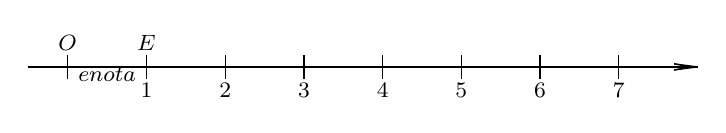
\begin{tikzpicture}
                        % \clip (0,0) rectangle (14.000000,10.000000);
                        {\footnotesize
                        
                        % Drawing segment a b
                        \draw [line width=0.016cm] (0.500000,0.500000) -- (9.000000,0.500000);%
                        
                        % Drawing arrow a b 1.00
                        \draw [line width=0.016cm] (8.702567,0.539158) -- (9.000000,0.500000);%
                        \draw [line width=0.016cm] (8.702567,0.539158) -- (8.900856,0.500000);%
                        \draw [line width=0.016cm] (8.702567,0.460842) -- (9.000000,0.500000);%
                        \draw [line width=0.016cm] (8.702567,0.460842) -- (8.900856,0.500000);%
                        
                        % Drawing segment c d
                        \draw [line width=0.016cm] (1.000000,0.350000) -- (1.000000,0.650000);%
                        
                        % Drawing segment e f
                        \draw [line width=0.016cm] (2.000000,0.350000) -- (2.000000,0.650000);%
                        
                        % Drawing segment g h
                        \draw [line width=0.016cm] (3.000000,0.350000) -- (3.000000,0.650000);%
                        
                        % Drawing segment i j
                        \draw [line width=0.016cm] (4.000000,0.350000) -- (4.000000,0.650000);%
                        
                        % Drawing segment k l
                        \draw [line width=0.016cm] (5.000000,0.350000) -- (5.000000,0.650000);%
                        
                        % Drawing segment m n
                        \draw [line width=0.016cm] (6.000000,0.350000) -- (6.000000,0.650000);%
                        
                        % Drawing segment o p
                        \draw [line width=0.016cm] (7.000000,0.350000) -- (7.000000,0.650000);%
                        
                        % Drawing segment r s
                        \draw [line width=0.016cm] (8.000000,0.350000) -- (8.000000,0.650000);%
                        
                        % Marking point O
                        \draw (1.000000,0.600000) node [anchor=south] { $O$ };%
                        
                        % Marking point E
                        \draw (2.000000,0.600000) node [anchor=south] { $E$ };%
                        
                        % Marking point 1
                        \draw (2.000000,0.400000) node [anchor=north] { $1$ };%
                        
                        % Marking point 2
                        \draw (3.000000,0.400000) node [anchor=north] { $2$ };%
                        
                        % Marking point 3
                        \draw (4.000000,0.400000) node [anchor=north] { $3$ };%
                        
                        % Marking point 4
                        \draw (5.000000,0.400000) node [anchor=north] { $4$ };%
                        
                        % Marking point 5
                        \draw (6.000000,0.400000) node [anchor=north] { $5$ };%
                        
                        % Marking point 6
                        \draw (7.000000,0.400000) node [anchor=north] { $6$ };%
                        
                        % Marking point 7
                        \draw (8.000000,0.400000) node [anchor=north] { $7$ };%
                        
                        % Marking point {enota}
                        \draw (1.500000,0.600000) node [anchor=north] { ${enota}$ };%
                        }
                    \end{tikzpicture}
                        
                \end{figure}}

            \end{block}}

            \only<4->{\begin{block}{}
                Vsako število zapišemo s \textbf{številko}. 
                Za zapis številke uporabljamo \textbf{števke}. Te so $0, 1, 2, 3, 4, 5, 6, 7, 8, 9$.
            \end{block}}

            \only<5->{\begin{block}{}
                Posamezne števke večmestnega števila od desne proti levi predstavljajo: \textbf{enice}, \textbf{desetice}, \textbf{stotice}, \textbf{tisočice}, ...
            \end{block}}

            \only<6->{\begin{block}{}
                Število, ki je zapisano s črkovnimi oznakami števk označimo s črto nad zapsiom črkovne oznake.
                \only<7->{$$ \overline{xy}=10x+y \quad \quad \quad \overline{xyz}=100x+10y+z$$}
            \end{block}}

            
        \end{frame}

        \begin{frame}
            \frametitle{Operacije v množici $\mathbb{N}$}

            \only<2->{\begin{alertblock}{Seštevanje}
                \only<3->{Poljubnima naravnima številoma $x$ in $y$ priredimo \textbf{vsoto} $\mathbf{x+y}$.}
            \end{alertblock}}

            \only<4->{\begin{block}{}
                Število $x$ oziroma $y$ imenujemo \textbf{seštevanec} ali \textbf{sumand} ali \textbf{člen}. 

                \only<5->{Število $x+y$ pa imenujemo \textbf{vsota} ali \textbf{summa}. }

            \only<6->{\begin{figure}
                \begin{tikzpicture}
                    % \clip (0,0) rectangle (14.000000,10.000000);
                    {\footnotesize
                    
                    % Drawing segment a b
                    \draw [line width=0.016cm] (5.000000,0.500000) -- (5.000000,2.500000);%
                    
                    % Drawing segment b d
                    \draw [line width=0.016cm] (5.000000,2.500000) -- (7.000000,2.500000);%
                    
                    % Drawing segment c d
                    \draw [line width=0.016cm] (7.000000,0.500000) -- (7.000000,2.500000);%
                    
                    % Drawing segment c a
                    \draw [line width=0.016cm] (7.000000,0.500000) -- (5.000000,0.500000);%
                    
                    % Drawing segment e f
                    \draw [line width=0.016cm] (7.000000,1.500000) -- (9.000000,1.500000);%
                    
                    % Drawing arrow e f 1.00
                    \draw [line width=0.016cm] (8.702567,1.539158) -- (9.000000,1.500000);%
                    \draw [line width=0.016cm] (8.702567,1.539158) -- (8.900856,1.500000);%
                    \draw [line width=0.016cm] (8.702567,1.460842) -- (9.000000,1.500000);%
                    \draw [line width=0.016cm] (8.702567,1.460842) -- (8.900856,1.500000);%
                    
                    % Drawing segment g h
                    \draw [line width=0.016cm] (2.500000,1.000000) -- (5.000000,1.000000);%
                    
                    % Drawing segment i j
                    \draw [line width=0.016cm] (2.500000,2.000000) -- (5.000000,2.000000);%
                    
                    % Drawing arrow g h 1.00
                    \draw [line width=0.016cm] (4.702567,1.039158) -- (5.000000,1.000000);%
                    \draw [line width=0.016cm] (4.702567,1.039158) -- (4.900856,1.000000);%
                    \draw [line width=0.016cm] (4.702567,0.960842) -- (5.000000,1.000000);%
                    \draw [line width=0.016cm] (4.702567,0.960842) -- (4.900856,1.000000);%
                    
                    % Drawing arrow i j 1.00
                    \draw [line width=0.016cm] (4.702567,2.039158) -- (5.000000,2.000000);%
                    \draw [line width=0.016cm] (4.702567,2.039158) -- (4.900856,2.000000);%
                    \draw [line width=0.016cm] (4.702567,1.960842) -- (5.000000,2.000000);%
                    \draw [line width=0.016cm] (4.702567,1.960842) -- (4.900856,2.000000);%
                    
                    % Marking point {vsota}
                    \draw (8.000000,1.500000) node [anchor=south] { ${vsota}$ };%
                    
                    % Marking point {summa}
                    \draw (8.000000,1.500000) node [anchor=north] { ${summa}$ };%
                    
                    % Marking point {se�tevanec}
                    \draw (3.750000,1.000000) node [anchor=south] { ${seštevanec}$ };%
                    
                    % Marking point {sumand}
                    \draw (3.750000,1.000000) node [anchor=north] { ${sumand}$ };%
                    
                    % Marking point {se�tevanec}
                    \draw (3.750000,2.000000) node [anchor=south] { ${seštevanec}$ };%
                    
                    % Marking point {sumand}
                    \draw (3.750000,2.000000) node [anchor=north] { ${sumand}$ };%
                    
                    % Drawing segment x y
                    \draw [line width=0.032cm] (6.000000,1.000000) -- (6.000000,2.000000);%
                    
                    % Drawing segment z w
                    \draw [line width=0.032cm] (5.500000,1.500000) -- (6.500000,1.500000);%
                    }
                    \end{tikzpicture}
                    
            \end{figure}}


            \end{block}}


            \only<7->{\begin{block}{}
                Vsota naravnih števil je naravno število: $x, y \in \mathbb{N} \Rightarrow x+y \in \mathbb{N}$.

            \end{block}}

        \end{frame}

        \begin{frame}
            \only<2->{\begin{alertblock}{Množenje}
                \only<3->{Poljubnima naravnima številoma $x$ in $y$ priredimo \textbf{produkt} $\mathbf{x\cdot y}$.}
            \end{alertblock}}

            \only<4->{\begin{block}{}
                Število $x$ oziroma $y$ imenujemo \textbf{množenec} ali \textbf{faktor}. 

                \only<5->{Število $x\cdot y$ pa imenujemo \textbf{zmnožek} ali \textbf{produkt}. }

                \only<6->{\begin{figure}
                \begin{tikzpicture}
                    % \clip (0,0) rectangle (14.000000,10.000000);
                    {\footnotesize
                    
                    % Drawing segment a b
                    \draw [line width=0.016cm] (5.000000,0.500000) -- (5.000000,2.500000);%
                    
                    % Drawing segment b d
                    \draw [line width=0.016cm] (5.000000,2.500000) -- (7.000000,2.500000);%
                    
                    % Drawing segment c d
                    \draw [line width=0.016cm] (7.000000,0.500000) -- (7.000000,2.500000);%
                    
                    % Drawing segment c a
                    \draw [line width=0.016cm] (7.000000,0.500000) -- (5.000000,0.500000);%
                    
                    % Drawing segment e f
                    \draw [line width=0.016cm] (7.000000,1.500000) -- (9.000000,1.500000);%
                    
                    % Drawing arrow e f 1.00
                    \draw [line width=0.016cm] (8.702567,1.539158) -- (9.000000,1.500000);%
                    \draw [line width=0.016cm] (8.702567,1.539158) -- (8.900856,1.500000);%
                    \draw [line width=0.016cm] (8.702567,1.460842) -- (9.000000,1.500000);%
                    \draw [line width=0.016cm] (8.702567,1.460842) -- (8.900856,1.500000);%
                    
                    % Drawing segment g h
                    \draw [line width=0.016cm] (2.500000,1.000000) -- (5.000000,1.000000);%
                    
                    % Drawing segment i j
                    \draw [line width=0.016cm] (2.500000,2.000000) -- (5.000000,2.000000);%
                    
                    % Drawing arrow g h 1.00
                    \draw [line width=0.016cm] (4.702567,1.039158) -- (5.000000,1.000000);%
                    \draw [line width=0.016cm] (4.702567,1.039158) -- (4.900856,1.000000);%
                    \draw [line width=0.016cm] (4.702567,0.960842) -- (5.000000,1.000000);%
                    \draw [line width=0.016cm] (4.702567,0.960842) -- (4.900856,1.000000);%
                    
                    % Drawing arrow i j 1.00
                    \draw [line width=0.016cm] (4.702567,2.039158) -- (5.000000,2.000000);%
                    \draw [line width=0.016cm] (4.702567,2.039158) -- (4.900856,2.000000);%
                    \draw [line width=0.016cm] (4.702567,1.960842) -- (5.000000,2.000000);%
                    \draw [line width=0.016cm] (4.702567,1.960842) -- (4.900856,2.000000);%
                    
                    % Marking point {zmno�ek}
                    \draw (8.000000,1.500000) node [anchor=south] { ${zmnožek}$ };%
                    
                    % Marking point {produkt}
                    \draw (8.000000,1.500000) node [anchor=north] { ${produkt}$ };%
                    
                    % Marking point {mno�enec}
                    \draw (3.750000,1.000000) node [anchor=south] { ${množenec}$ };%
                    
                    % Marking point {faktor}
                    \draw (3.750000,1.000000) node [anchor=north] { ${faktor}$ };%
                    
                    % Marking point {mno�enec}
                    \draw (3.750000,2.000000) node [anchor=south] { ${množenec}$ };%
                    
                    % Marking point {faktor}
                    \draw (3.750000,2.000000) node [anchor=north] { ${faktor}$ };%
                    
                    % Drawing circle k
                    \draw [line width=0.016cm] (6.000000,1.500000) circle (0.100000);%
                    
                    % Filling circle k
                    \fill (6.000000,1.500000) circle (0.100000);%
                    }
                    \end{tikzpicture}
                    
            \end{figure}}

            \end{block}}


            \only<7->{\begin{block}{}
                Produkt naravnih števil je naravno število: $x, y \in \mathbb{N} \Rightarrow x\cdot y \in \mathbb{N}$.
            \end{block}}

            \only<8->{\begin{block}{}
                Število $\mathbf{1}$ je \textbf{nevtralni element} za mmnoženje: $1\cdot x = x$.
            \end{block}}

        \end{frame}

        \begin{frame}
            

            \only<2->{\begin{alertblock}{Odštevanje}
                \only<3->{Številoma $x$ in $y$, pri čemer je $x$ večje od $y$ ($x>y$), priredimo \textbf{razliko} $\mathbf{x-y}$.}
            \end{alertblock}}

            \only<4->{\begin{block}{}
                Število $x$ imenujemo \textbf{zmanjševanec} ali \textbf{minuend}, število $y$  pa imenujemo \textbf{odštevanec} ali \textbf{subtrahend}. 

                \only<5->{Številu $x-y$ rečemo \textbf{razlika} ali \textbf{diferenca}. }

                \only<6->{\begin{figure}
                    \begin{tikzpicture}
                        % \clip (0,0) rectangle (14.000000,10.000000);
                        {\footnotesize
                        
                        % Drawing segment a b
                        \draw [line width=0.016cm] (5.000000,0.500000) -- (5.000000,2.500000);%
                        
                        % Drawing segment b d
                        \draw [line width=0.016cm] (5.000000,2.500000) -- (7.000000,2.500000);%
                        
                        % Drawing segment c d
                        \draw [line width=0.016cm] (7.000000,0.500000) -- (7.000000,2.500000);%
                        
                        % Drawing segment c a
                        \draw [line width=0.016cm] (7.000000,0.500000) -- (5.000000,0.500000);%
                        
                        % Drawing segment e f
                        \draw [line width=0.016cm] (7.000000,1.500000) -- (9.000000,1.500000);%
                        
                        % Drawing arrow e f 1.00
                        \draw [line width=0.016cm] (8.702567,1.539158) -- (9.000000,1.500000);%
                        \draw [line width=0.016cm] (8.702567,1.539158) -- (8.900856,1.500000);%
                        \draw [line width=0.016cm] (8.702567,1.460842) -- (9.000000,1.500000);%
                        \draw [line width=0.016cm] (8.702567,1.460842) -- (8.900856,1.500000);%
                        
                        % Drawing segment g h
                        \draw [line width=0.016cm] (2.500000,1.000000) -- (5.000000,1.000000);%
                        
                        % Drawing segment i j
                        \draw [line width=0.016cm] (2.500000,2.000000) -- (5.000000,2.000000);%
                        
                        % Drawing arrow g h 1.00
                        \draw [line width=0.016cm] (4.702567,1.039158) -- (5.000000,1.000000);%
                        \draw [line width=0.016cm] (4.702567,1.039158) -- (4.900856,1.000000);%
                        \draw [line width=0.016cm] (4.702567,0.960842) -- (5.000000,1.000000);%
                        \draw [line width=0.016cm] (4.702567,0.960842) -- (4.900856,1.000000);%
                        
                        % Drawing arrow i j 1.00
                        \draw [line width=0.016cm] (4.702567,2.039158) -- (5.000000,2.000000);%
                        \draw [line width=0.016cm] (4.702567,2.039158) -- (4.900856,2.000000);%
                        \draw [line width=0.016cm] (4.702567,1.960842) -- (5.000000,2.000000);%
                        \draw [line width=0.016cm] (4.702567,1.960842) -- (4.900856,2.000000);%
                        
                        % Marking point {razlika}
                        \draw (8.000000,1.500000) node [anchor=south] { ${razlika}$ };%
                        
                        % Marking point {diferenca}
                        \draw (8.000000,1.500000) node [anchor=north] { ${diferenca}$ };%
                        
                        % Marking point {od�tevanec}
                        \draw (3.750000,1.000000) node [anchor=south] { ${odštevanec}$ };%
                        
                        % Marking point {subtrahend}
                        \draw (3.750000,1.000000) node [anchor=north] { ${subtrahend}$ };%
                        
                        % Marking point {zmanj�evanec}
                        \draw (3.750000,2.000000) node [anchor=south] { ${zmanjševanec}$ };%
                        
                        % Marking point {minuend}
                        \draw (3.750000,2.000000) node [anchor=north] { ${minuend}$ };%
                        
                        % Drawing segment z w
                        \draw [line width=0.032cm] (5.500000,1.500000) -- (6.500000,1.500000);%
                        }
                        \end{tikzpicture}
                        
            \end{figure}}
        \end{block}}

            \only<7->{\begin{block}{}
                Razlika je število, ki ga moramo prišteti številu $y$, da dobimo število $x$.
                \only<8->{$$ (x-y)+y=x $$}
            \end{block}}

        \end{frame}

        \begin{frame}
            \only<2->{\begin{block}{}
                Seštevanje in množenje sta \textit{dvočleni notranji operaciji} v množici naravnih števil $\mathbb{N}$.

                \only<3->{Odštevanje pa ni notranja operacija v množici naravnih števil $\mathbb{N}$.}
            \end{block}}

            \only<4->{\begin{block}{Vrstni red operacij}
                \only<5->{Prednost pri računanju imajo \textbf{oklepaji} (najprej najbolj notranji),} 
                \only<6->{nato sledi \textbf{množenje},}
                \only<7->{na koncu pa imamo še \textbf{seštevanje} in \textbf{odštevanje}.}
            \end{block}}

            \only<8->{\begin{block}{}
                Kadar v izrazu nastopajo enakovredne računske operacije, računamo od leve proti desni.
            \end{block}}

            \only<9->{\begin{block}{}
                Pri množenju količin, ki so označene s črkovnimi oznakami, piko, ki označuje operacijo množenja ponavadi opustimo.
                \only<10->{$$ x\cdot y = xy$$}
            \end{block}}


        \end{frame}

        \begin{frame}
            \frametitle{Osnovni računski zakoni v $\mathbb{N}$}

            \only<2->{\begin{block}{Komutativnost seštevanja -- zakon o zamenjavi členov}
                \only<3->{$$ \mathbf{x+y=y+x}$$}
                \only<4->{Vsota ni odvisna od vrstnega reda seštevanja.}
            \end{block}}

            \only<5->{\begin{block}{Asociativnost seštevanja -- zakon o poljubnem združevanju členov}
                \only<6->{$$ \mathbf{(x+y)+z=x+(y+z)}$$}
                \only<7->{Vsota več kot dveh sumandov ni odvisna od združevanja po dveh sumandov.}
            \end{block}}

        \end{frame}

        \begin{frame}


            \only<2->{\begin{block}{Komutativnost množenja -- zakon o zamenjavi faktorjev}
                \only<3->{$$ \mathbf{x\cdot y=y\cdot x}$$}
                \only<4->{Produkt ni odvisen od vrstnega reda faktorjev.}
            \end{block}}

            \only<5->{\begin{block}{Asociativnost množenja -- zakon o poljubnem združevanju faktorjev}
                \only<6->{$$ \mathbf{(x\cdot y)\cdot z=x\cdot (y\cdot z)}$$}
                \only<7->{Produkt več kot dveh sumandov ni odvisen od združevanja faktorjev.}
            \end{block}}

            \only<8->{\begin{block}{Distributivnost -- zakon o razčlenjevanju}
                \only<9->{$$ \mathbf{x\cdot z+y\cdot z = (x+y)\cdot z} $$}
                \only<10->{Če to beremo iz desne proti levi, rečemu tudi \textit{pravilo izpostavljanja skupnega faktorja}.}
            \end{block}}

        \end{frame}

        \begin{frame}
            \only<2->{\begin{exampleblock}{Naloga}
                Izračunajte.
                \only<3->{\begin{itemize}
                    \item $(1+2\cdot 7)+3\cdot(2\cdot 2+7)$ \\ ~
                    \item $3\cdot(2+3\cdot 5)\cdot(2+1)$ \\ ~
                    \item $7+(2+6\cdot 3)+(8+4\cdot 5)$ \\ ~
                    \item $11\cdot 4+(12-6)\cdot 5$ \\ ~
                    \item $8+2\cdot(3+7)-15$ \\ ~
                    \item $37-5\cdot(10-3)$ \\ ~
                \end{itemize}}
            \end{exampleblock}}
        \end{frame}

        \begin{frame}
            \only<2->{\begin{exampleblock}{Naloga}
                Hitro izračunajte.
                \only<3->{\begin{itemize}
                    \item $45+37+15$ 
                    \item $108+46-28$
                    \item $5\cdot 13\cdot 8$
                    \item $4\cdot 7\cdot 25$
                    \item $(7+3)\cdot 2\cdot 5$
                    \item $15\cdot(4+6)\cdot 2$
                    \item $3\cdot 5+7\cdot 5$
                    \item $8\cdot 12+6\cdot 8$
                \end{itemize}}
            \end{exampleblock}}
        \end{frame}

        \begin{frame}
            \only<2->{\begin{exampleblock}{Naloga}
                Zapišite račun glede na besedilo in izračunajte.
                \only<3->{\begin{itemize}
                    \item Produktu števil $12$ in $27$ odštejte razliko števil $19$ in $11$. \\ ~
                    \item Vsoti produkta $4$ in $12$ ter produkta $5$ in $16$ odštejte $8$. \\ ~
                    \item Vsoto števil $42$ in $23$ pomnožite z razliko števil $58$ in $29$. \\ ~
                    \item Produkt števil $14$ in $17$ pomnožite z vsoto števil $5$ in $16$. \\ ~ \\ ~
                \end{itemize}}
            \end{exampleblock}}
        \end{frame}

        \begin{frame}
            \only<2->{\begin{exampleblock}{Naloga}
                Rešite besedilno nalogo.
                \only<3->{\begin{itemize}
                    \item V trgovini kupimo tri litre mleka in štiri čokoladne pudinge v prahu. Če stane liter mleka $95$ centov,
                        čokoladni puding v prahu pa $24$ centov, koliko moramo plačati? \\ ~ \\ ~ \\ ~ \\ ~
                    \item Manca bo kuhala rižoto za štiri otroke in šest odraslih. Za otroško porcijo rižote zadošča $45~g$ riža,
                        za odraslo pa $75~g$. Koliko riža mora dati kuhati za rižoto? \\ ~ \\ ~ \\ ~ \\ ~
                \end{itemize}}
            \end{exampleblock}}
        \end{frame}

\subsection{Cela števila}
        \begin{frame}
            \frametitle{Cela števila}

                \only<2->{\begin{alertblock}{Množica celih števil}
                    \only<3->{$$\mathbf{\mathbb{Z} = \{\ldots, -2, -1, 0, 1, 2, 3, \ldots\}}$$}
                \end{alertblock}}

                \only<4->{\begin{block}{}
                    Množica celih števil $\mathbb{Z}$ je definirana kot unija treh množic:
                        \begin{itemize}
                            \item<5-> množica \textbf{pozitivnih celih števil} ($\mathbb{Z}^+$) -- naravna števila $\mathbb{N}$;
                            \item<6-> \textbf{število 0};
                            \item<7-> množica \textbf{negativnih celih števil} ($\mathbb{Z}^-$) -- nasprotna števila vseh naravnih števil.
                        \end{itemize}
                      \only<8->{$$\mathbb{Z} = \mathbb{Z}^- \cup \{0\} \cup \mathbb{Z}^+$$}

                \end{block}}

                \only<9->{\begin{block}{}
                    \textbf{Nasprotna vrednost} števila $n$ je število $-n$.
                \end{block}}
        \end{frame}

        \begin{frame}
            \frametitle{Operacije v množici $\mathbb{Z}$}

            \only<2->{\textbf{\large{Seštevanje}}}

            \only<3->{\begin{block}{}
                $$\mathbf{x+0=x}; ~\forall x\in\mathbb{Z}$$
                \only<4->{Število $0$ je \textbf{nevtralni element} pri seštevanju.}
            \end{block}}

            \only<5->{\begin{block}{}
                $$\mathbf{x+(-x)=0}; ~\forall x\in\mathbb{Z} $$
                \only<6->{Vsota celega števila in njemu nasprotnega števila je enaka $0$.}
            \end{block}}

            \only<7->{\begin{block}{}
                $$\mathbf{-(-x)=x}; ~\forall x\in\mathbb{Z}$$
                \only<8->{Nasprotna vrednost nasprotne vrednosti je enaka prvotni vrednosti.}
            \end{block}}
        \end{frame}


        \begin{frame}

            \only<2->{\begin{block}{}
                Vsota dveh pozitivnih števil je pozitivno število, vsota dveh negativnih števil pa je negativno število.
            \end{block}}

            \only<3->{\begin{block}{}
                $$\mathbf{-x+(-y)=-(x+y)}$$
                \only<4->{Vsota nasprotnih vrednosti je enaka nasprotni vrednosti vsote.}
            \end{block}}

            \only<5->{\begin{block}{}
                Naj bosta $x$ in $y$ naravni števili. Vsota pozitivnega števila $x$ in negativnega števila $-y$ je:
                \begin{itemize}
                    \item<6-> pozitivno število, če je $x>y$ in
                    \item<7-> negativno število, če je $x<y$.
                \end{itemize}
            \end{block}}
        \end{frame}


        \begin{frame}
            \only<2->{\textbf{\large{Odštevanje}}}

            \only<3->{\begin{block}{}
                Razlika $x-y$ dveh pozitivnih števil $x$ in $y$ je:
                \begin{itemize}
                    \item<4-> pozitivno število, če je $x>y$ in 
                    \item<5-> negativno število, če je $x<y$.
                \end{itemize}
            \end{block}}

            \only<6->{\begin{block}{}
                Razlika dveh negativnih števil $(-x)-(-y)$ je:
                \begin{itemize}
                    \item<7-> pozitvno število, če je $x<y$ in 
                    \item<8-> negativno število, če je $x>y$.
                \end{itemize}
            \end{block}}

            \only<9->{\begin{block}{}
                Razlika pozitivnega števila $x$ in negativnega števila $-y$ je pozitvno število.
            \end{block}}


            \only<10->{\begin{alertblock}{}
                \textit{Odštevanje v množici $\mathbb{Z}$ je prištevanje nasprotne vrednosti.}
                \only<11->{$$\mathbf{x-y=x+(-y)} $$}
            \end{alertblock}}
        \end{frame}

        \begin{frame}
            \only<2->{\textbf{\large{Množenje}}}

            \only<3->{\begin{block}{}
                $$\mathbf{1\cdot x=x}; ~\forall x\in\mathbb{Z}$$
                \only<4->{Število $1$ je \textbf{nevtralni element} za množenje.}
            \end{block}}

            \only<5->{\begin{block}{}
                $$\mathbf{(-1)\cdot x=-x}; ~\forall x\in\mathbb{Z}$$
                \only<6->{Pri množenju celega števila $x$ z $-1$ dobimo nasprotno število $-x$.}
            \end{block}}

            \only<7->{\begin{block}{}
                $$\mathbf{0\cdot x=0}; ~\forall x\in\mathbb{Z}$$
                \only<8->{Rezultat množenja števila s številom $0$ je enak $0$.}
            \end{block}}

        \end{frame}

        \begin{frame}


            \only<2->{\begin{block}{}
                $$\mathbf{(-x)(-y)=xy}$$
                \only<3->{Produkt sodo mnogo negativnih števil je pozitivno število.}
            \end{block}}

            \only<4->{\begin{block}{}
                $$\mathbf{-x\cdot y=-(xy)}$$
                \only<5->{$$\mathbf{x(-y)=-(xy)}$$}
                \only<6->{Produkt pozitivnega in negativnega števila je negativno število.}
            \end{block}}

            \only<7->{\begin{block}{}
                Produkt liho mnogo negativnih faktorjev je negativno število.
            \end{block}}

            \only<8->{\begin{block}{}
                Seštevanje, odštevanje in množenje so v množici $\mathbb{Z}$ dvočlene notranje operacije.
            \end{block}}
        \end{frame}


        \begin{frame}
            \frametitle{Osnovni računski zakoni v $\mathbb{Z}$}

            \begin{columns}[T]
                \column{0.48\textwidth}
                \only<2->{\begin{block}{Komutativnost seštevanja}
                    \only<3->{$$ \mathbf{x+ y=y+ x}$$}
                \end{block}}
    
                \only<4->{\begin{block}{Asociativnost seštevanja}
                    \only<5->{$$ \mathbf{(x+ y)+ z=x+ (y+ z)}$$}
                \end{block}}

                \column{0.48\textwidth}

                \only<6->{\begin{block}{Komutativnost množenja}
                    \only<7->{$$ \mathbf{x\cdot y=y\cdot x}$$}
                \end{block}}
    
                \only<8->{\begin{block}{Asociativnost množenja}
                    \only<9->{$$ \mathbf{(x\cdot y)\cdot z=x\cdot (y\cdot z)}$$}
                \end{block}}
            \end{columns}

    
                \only<10->{\begin{block}{Distributivnost seštevanja in množenja ter odštevanja in množenja}
                    \only<11->{$$ \mathbf{x\cdot z+y\cdot z = (x+y)\cdot z} $$}
                    \only<12->{$$ \mathbf{x\cdot z-y\cdot z = (x-y)\cdot z} $$}

                \end{block}}
    
        \end{frame}


        \begin{frame}
            \only<2->{\begin{exampleblock}{Naloga}
                Izračunajte.
                \only<3->{\begin{itemize}
                    \item $17-13-2+10$ \\ ~
                    \item $50+11-32-14$ \\ ~
                    \item $3+((5+2(7-9))\cdot 2-1)$ \\ ~
                    \item $(2-5(6-10))\cdot(5-2(7-5))$ \\ ~
                    \item $9(11-3)+7(10-15)$ \\ ~
                    \item $8+9(11-18)-2\cdot 5$ \\ ~
                \end{itemize}}
            \end{exampleblock}}
        \end{frame}

        \begin{frame}
            \only<2->{\begin{exampleblock}{Naloga}
                Spretno izračunajte.
                \only<3->{\begin{itemize}
                    \item $7\cdot 8-12\cdot 8$ \\ ~
                    \item $5\cdot 18+9\cdot 5-5\cdot 2$ \\ ~
                    \item $8\cdot(4-9)\cdot 2$ \\ ~
                    \item $5\cdot 3\cdot (12-8)$ \\ ~
                    \item $(15-6)(12-3\cdot 4)$ \\ ~
                \end{itemize}}
            \end{exampleblock}}
        \end{frame}

        \begin{frame}
            \only<2->{\begin{exampleblock}{Naloga}
                Rešite besedilne naloge.
                \only<3->{\begin{itemize}
                    \item V hotelu imajo na voljo osemnajst enoposteljnih, štiriintrideset dvoposteljnih in petindevetdeset triposteljnih sob.
                        Koliko ljudi lahko še prespi v hotelu, če je v njem že sto triinštirideset gostov? \\ ~ \\ ~ \\ ~
                    \item Pohod na bližnji hrib traja tri ure. Koliko minut moramo še hoditi, če smo na poti že $145$ minut? \\ ~ \\ ~ \\ ~ \\
                \end{itemize}}
            \end{exampleblock}}
        \end{frame}

        \begin{frame}

            \only<2->{\begin{exampleblock}{Naloga}
                \only\begin{itemize}
                    \item S Ptuja in iz Postojne (razdalja med njima je približno $190~km$) sočasno odpeljeta dva motorista drug proti drugemu.
                        En vozi povprečno $40~km/h$, drugi pa $5~km/h$ manj. Kolikšna bo razdalja med njima po dveh urah vožnje? \\ ~ \\ ~ \\ ~
                \end{itemize}
            \end{exampleblock}}

            \only<3->{\begin{exampleblock}{Naloga}
                Zapišite enačbe in jih poenostavite.
                \only<4->{\begin{itemize}
                    \item Razlika petkratnika $a$ in $b$ je enaka trikratniku vsote štirikratnika $a$ in petkratnika $b$. \\ ~ \\
                    \item Vsota $x$ in dvakratnika $y$ je enaka razliki petkratnika $x$ in dvanajstkratnika $y$. \\ ~ \\ ~
                \end{itemize}}
            \end{exampleblock}}
        \end{frame}






\subsection{Urejenost naravnih in celih števil}

        \begin{frame}
            \frametitle{Urejenost naravnih in celih števil}

            \only<2->{\begin{alertblock}{}
                Številska množica je \textbf{urejena}, kadar lahko po velikosti primerjamo njena poljubna elementa.
            \end{alertblock}}

            \only<3->{\begin{block}{}
                Pri urejanju števil uporabljamo naslednje znake:
                \only<4->{\begin{table}
                    \centering
                    \addtolength{\tabcolsep}{6pt}
                    \renewcommand{\arraystretch}{1.4}                
                    \begin{tabular}{||c|c||} 
                        \hhline{|t:==:t|}
                                $\mathbf{<}$ & manjše / manj  \\ 
                        \hline
                                $\mathbf{>}$ & večje / več   \\ 
                        \hline
                                $\mathbf{\leq}$ & manjše ali enako / največ   \\ 
                        \hline
                                $\mathbf{\geq}$ & večje ali enako / vsaj, najmanj \\  
                        \hline
                                $\mathbf{=}$ & enako \\
                        \hhline{|b:==:b|}
                    \end{tabular}
                \end{table}}
            \end{block}}
        \end{frame}

        \begin{frame}
            \only<2->{\begin{block}{}
                Za poljubni števili $x,y\in\mathbb{Z}$ velja natanko ena izmed naslednjih možnosti: $x>y$, $x<y$ ali $x=y$.
            \end{block}}

            \only<3->{\begin{block}{}
                $$\mathbf{x>y \Leftrightarrow x-y>0}$$
                \only<4->{Slika števila $x$ leži na številski premici desno od slike števila $y$.}
            \end{block}}

            \only<5->{\begin{block}{}
                $$\mathbf{x<y \Leftrightarrow x-y<0}$$
                \only<6->{Slika števila $x$ leži na številski premici levo od slike števila $y$.}
            \end{block}}

            \only<7->{\begin{block}{}
                $$\mathbf{x=y \Leftrightarrow x-y=0}$$
                \only<8->{Slika števila $x$ sovpada s sliko števila $y$.}
            \end{block}}

        \end{frame}

        \begin{frame}
            \only<2->{\begin{block}{Pozitivna števila}
                \only<3->{V množici $\mathbb{Z}$ so pozitivna tista števila, ki so večja od števila $0$ 
                in njihove slike ležijo desno od izhodišča.}
            \end{block}}
            
            \only<4->{\begin{block}{Negativna števila}
                \only<5->{V množici $\mathbb{Z}$ so negativna tista števila, ki so manjša od števila $0$ 
                in njihove slike ležijo levo od izhodišča.}
            \end{block}}

            \only<6->{\begin{block}{}
                Vsako pozitivno celo število (vsako naravno število) je večje od katerega koli negativnega celega števila.
            \end{block}}

            \only<7->{\begin{block}{}
                Velja pa tudi:
                $$x\leq y \Leftrightarrow x-y\leq 0 $$
                \only<8->{$$x\geq y \Leftrightarrow x-y\geq 0 $$}
            \end{block}}
        \end{frame}


        \begin{frame}
            \only<2->{\begin{alertblock}{}
                Z relacijo \textit{biti manjši ali enak} je množica $\mathbb{Z}$ \textbf{linearno urejena}, 
                to pomeni, da veljajo:
            \end{alertblock}}
            
            \only<3->{\begin{block}{Refleksivnost}
                \only<4->{$$\forall x\in\mathbb{Z}: x\leq x$$}
            \end{block}}

            \only<5->{\begin{block}{Antisimetričnost}
                \only<6->{$$\forall x,y\in\mathbb{Z}: x\leq y \land y\leq x \Rightarrow x=y$$}
            \end{block}}

            \only<7->{\begin{block}{Tranzitivnost}
                \only<8->{$$\forall x,y,z\in\mathbb{Z}: x\leq y \land y\leq z \Rightarrow x\leq z$$}
            \end{block}}

            \only<9->{\begin{block}{Stroga sovisnost}
                \only<10->{$$\forall x,y\in\mathbb{Z}: x\leq y \lor y\leq x$$}
            \end{block}}

        \end{frame}

        \begin{frame}
            \only<2->{\begin{block}{Monotonost vsote}
                \only<3->{$$x<y \Rightarrow x+z<y+z \quad \quad x\leq y \Rightarrow x+z\leq y+z$$}
                \only<4->{Če na obeh straneh neenakosti prištejemo isto število, se neenakost ohrani.}
            \end{block}}

            \only<5->{\begin{block}{}
                $$x<y \land z>0 \Rightarrow x\cdot z<y\cdot z \quad \quad x\leq y \land z>0 \Rightarrow x\cdot z\leq y\cdot z$$
                \only<6->{Pri množenju neenakosti z negativnim številom se znak neenakosti ohrani.}
            \end{block}}

            \only<7->{\begin{block}{}
                $$x<y \land z<0 \Rightarrow x\cdot z>y\cdot z \quad \quad x\leq y \land z<0 \Rightarrow x\cdot z\geq y\cdot z$$
                \only<8->{Pri množenju neenakosti z negativnim številom se znak neenakosti obrne.}
            \end{block}}

            \only<9->{\begin{block}{}
                Obravnavane lastnosti veljajo tudi za relaciji $\geq$ in $>$.
            \end{block}}

        \end{frame}

        \begin{frame}

                \only<2->{\begin{exampleblock}{Naloga}
                    Uredite števila $3, -2, 5, -1, 0, -7, 6, -6$ po velikosti in jih predstavite na številski premici.
                \end{exampleblock}}

                \only<3->{\begin{exampleblock}{Naloga}
                    Uredite števila $104, -27, 35, -107, 36, -26, 25, -28, 81$ po velikosti.
                \end{exampleblock}}

                \only<4->{\begin{exampleblock}{Naloga}
                    Gladina Mrtvega morja leži v depresiji na $-423~m$ nadmorske višine, njegova največja globina pa je $378~m$.
                    Kolikšna je najmanjša nadmorska višina dna Mrtvega morja?
                \end{exampleblock}}

                \only<5->{\begin{exampleblock}{Naloga}
                    Za katera cela števila $x$ ima izraz $3x-5(x+2)$ večjo ali enako vrednost od izraza $4-(12+x)$?
                \end{exampleblock}}
    
        \end{frame}



% \chapter{Potence in izrazi}
\section{Potence z naravnim eksponentom}


            Potenca $\mathbf{x^n}$ z \textbf{osnovo}/\textbf{bazo} $x$ in \textbf{eksponentom}/\textbf{stopnjo} $n \in \mathbb{N}$, je produkt $n$ faktorjev enakih $x$.

            $$ \mathbf{x^n=\underbrace{x\cdot x\cdot \ldots \cdot x}_\text{n faktorjev}}  $$
        
            % \begin{figure}[H]
            %     \centering
                
            %     \begin{tikzpicture}[scale=0.75]

            %         \draw[thick] (0,0)--(2,0); 
            %         \fill[red!40] (3,0) rectangle (5,2);
            %         \draw[black,thick] (3,0) rectangle (5,2);
            %         \node at (1,0.15) {$x$};


            %         \fill[red!40] (6,0) rectangle (8,2);
            %         \fill[red!40] (7,2.5)--(6,2)--(8,2)--(9,2.5)--cycle;
            %         \fill[red!40] (8,0)--(9,0.5)--(9,2.5)--(8,2)--cycle;
            %         \node at (4,1) {$x^2$};


            %         \draw[black,thick] (6,0) rectangle (8,2);
            %         \draw[black,thick] (7,2.5)--(6,2)--(8,2)--(9,2.5)--cycle;
            %         \draw[black,thick] (8,0)--(9,0.5)--(9,2.5)--(8,2)--cycle;
            %         \node at (7,1) {$x^3$};
                
            %     \end{tikzpicture}
            % \end{figure}
    

    
    
        \section{Pravila za računanje s potencami}

                    Dve potenci z isto osnovo zmnožimo tako, da osnovo ohranimo, eksponenta pa seštejemo.

            $$ x^n \cdot x^m=\underbrace{(x\cdot x\cdot\ldots\cdot x)}_\text{n faktorjev}\cdot\underbrace{(x\cdot x\cdot\ldots\cdot x)}_\text{m faktorjev}=x^{n+m}$$
            
            Potenco potenciramo tako, da osnovo ohranimo, ekponenta pa zmnožimo.

            $$ (x^n)^m=\underbrace{\underbrace{(x\cdot x\cdot\ldots\cdot x)}_\text{n faktorjev}\cdot\underbrace{(x\cdot x\cdot\ldots\cdot x)}_\text{n faktorjev}\cdot\ldots\cdot\underbrace{(x\cdot x\cdot\ldots\cdot x)}_\text{n faktorjev}}_\text{m faktorjev}=x^{n\cdot m}$$
            
    

    
            Produkt dveh ali več števil potenciramo tako, da potenciramo posamezne faktorje in jih potem zmnožimo.

            $$ (xy)^n =\underbrace{(xy\cdot xy\cdot\ldots\cdot xy)}_\text{n faktorjev}=\underbrace{(x\cdot x\cdot\ldots\cdot x)}_\text{n faktorjev}\cdot\underbrace{(y\cdot y\cdot\ldots\cdot y)}_\text{n faktorjev}=x^n y^n$$
            

            Za naravne eksponente velja še:
            $$(-x)^{2n}=x^{2n}$$
            $$(-x)^{2n+1}=-x^{2n+1}$$

            $$(-1)^n=\begin{cases}
                1; &n=2k \\
                -1; &n=2k-1
            \end{cases}; k\in\mathbb{N}$$
\newline ~\newline
            
            \begin{naloga}
                    Števila $-3^2$, $(-4)^2$, $-2^4$, $(-1)^{2024}$, $(-2)^3$ in $(-3)^2$ uredite po velikosti od najmanjšega do največjega. 
            \end{naloga}

                \begin{naloga}
                    Poiščite podatke in jih zapišite na dva načina: s potenco in številom brez potence.
                    \begin{itemize}
                        \item Razdalja med Zemljo in Soncem
                        \item Zemljina masa
                        \item Masa Sonca
                        \item Število zvezd v naši Galaksiji
                    \end{itemize}
                \end{naloga}
    
                \begin{naloga}
                    Izračunajte.
                    \begin{itemize}
                        \item $(-3)^2+2^4$ 
                        \item $(5-3)^3+(-3)^2$ 
                        \item $(2^2+1)^2+(-3)^3+(-2)^4$ 
                        \item $(-1)^{2024}+((-2)^5+5^2-(7-3^2)^3)^2$ 
                        \item $-1^{2n-1}+(-1)^{2n-1}$ 
                    \end{itemize}
                \end{naloga}

                \begin{naloga}
                        Poenostavite izraz.
                    \begin{itemize}
                        \item $2^7\cdot 2^3$ 
                        \item $a^3\cdot a^{12}\cdot a^5$ 
                        \item $(2z)^3$ 
                        \item $(m^2\cdot m^4)^3$ 
                        \item $a^3+2a^3-6a^3$ 
                        \item $x^2\cdot x^4+(-2x^3)^2-2(-x)^6$ 
                    \end{itemize}
                \end{naloga}

                
        \begin{naloga}
            Izračunajte, rezultat zapišite s potenco.
            \begin{itemize}
                \item $2\cdot 10^3\cdot 3\cdot 10^2\cdot 5\cdot 10^6$ 
                \item $(10^3)^2\cdot5\cdot 10^4\cdot 2\cdot 10^3$ 
                \item $(-2)^3\cdot 2^7$ 
                \item $-2^3\cdot (-2)^4\cdot 2^3$ 
                \item $2^3\cdot(-3)^2\cdot 6^4\cdot 3$ 
                \item $(-3)^3\cdot(-7)^2\cdot 21^7\cdot 7$ 
            \end{itemize}
        \end{naloga}

        \begin{naloga}
            Poenostavite.
            \begin{itemize}
                \item $2^3\cdot 3^4\cdot(2^4\cdot 3^2)^5$ 
                \item $(5^2\cdot 7)^3\cdot 5^2\cdot 7^3$ 
                \item $(-2^3\cdot 3^5)^4\cdot 2^6\cdot 3^5$ 
                \item $(-4)^2\cdot(-7)^{13}\cdot (-28)^5\cdot (-7^2)^3$ 
                \item $-6^2\cdot(-3)^2\cdot 8^5\cdot (-3^2)^3$ 
            \end{itemize}
        \end{naloga}

        \begin{naloga}
            Poenostavite.
            \begin{itemize}
                \item $a^3\cdot b^2\cdot a^7\cdot b^3\cdot b^5$ 
                \item $4x^4\cdot(2x^3)^2$ 
                \item $(k^3\cdot 2h^5)^2$ 
                \item $(x^2y^4)^2\cdot (x^3y)^3$ 
                \item $(a^2b^5)^3(ab^3)^2$ 
                \item $x^2y^3(x^3y^6)^2$ 
            \end{itemize}
        \end{naloga}

    
        \begin{naloga}
            Poenostavite.
            \begin{itemize}
                \item $2^3\cdot x^2\cdot 3^2\cdot(-x)^6$ 
                \item $(-a^3b)^4(-a^2b^5a^3)^3$ 
                \item $(2s^2\cdot(-s^2)^5)^5$ 
                \item $(-2(z^4)^2(-2z)^3z^5)^3$ 
                \item $(-3ab^2)^3(-a^4b^2(a^3)^5)^2(ab^3)^2$ 
                \item $(xy^2z)^3(x^3(-y^2)^5(-z))^3(x^2y^3(-z^2)^3)$ 
            \end{itemize}
        \end{naloga}

        \begin{naloga}
            Odpravite oklepaje in poenostavite, če je mogoče.
            \begin{itemize}
                \item $a^n\cdot a^{n+2}\cdot(-a)^3$ \\ ~
                \item $(-x^n)^4\cdot x^2$ 
                \item $a^n\cdot(a^2-a^3+2)$ 
                \item $(x^2+3x^n-5)\cdot x^{n+1}$ 
            \end{itemize}
        \end{naloga}


        \begin{naloga}
            Poenostavite.
            \begin{itemize}
                \item $(2s(g^2)^2)^2-3(s^4g)g^7$ 
                \item $(-4x^2xy^3)^2+(xy)^5(-2^3xy)$
                \item $a^2(a^3-b^2)-a^5+(-a)^2b^2$ 
                \item $(p^2(q^3)^2)^2-2p^4q^{12}+7(-p^3p)(q^4)^3-(-2)^3(pq^3)^4$ 
            \end{itemize}
        \end{naloga}

        \begin{naloga}
            Poenostavite.
            \begin{itemize}
                \item $5a^{n+1}+4a^{n+1}-6a^{n+1}$ 
                \item $3x^{n+2}+5x^n\cdot x^2+2x\cdot x^{n+1}$
                \item $3^{5x}\cdot 9^x-3^{7x}+27^x\cdot 9^{2x}$ 
                \item $4^{2y}+3\cdot(2^y)^4-5\cdot 8^y\cdot 2^y$ 
                \item $5^p\cdot 125^p\cdot 25^p+2(5^p)^6-4\cdot 25^{3p}$ 
            \end{itemize}
        \end{naloga}




\newpage
        \section{Večkratniki}

        
            
            
                \textbf{Večkratnik} ali tudi \textbf{$k$-kratnik} števila $x$ je vsota $k$ enakih sumandov $x$:
                    $${k\cdot x=\underbrace{x+x+\ldots+x}_\text{$k$ sumandov}}.$$
            
    
            
                Vse večkratnike števila $x$ dobimo tako, da število $x$ zapored pomnožimo z vsemi celimi števili:
                $$\left\{\ldots,-5x, -4x, -3x, -2x, -x, 0, x, 2x, 3x, 4x, 5x, \ldots\right\}=\left\{kx;\ k,x\in\mathbb{Z}\right\}=x\mathbb{Z}. $$
            
    
            
                Število $\mathbf{k}$ je \textbf{koeficient} števila oziroma spremenljivke $x$.
            
        
    
        \section{Algebrski izrazi}
    
        
    
            
                \textbf{Algebrski izraz} ali \textbf{izraz} je smiseln zapis sestavljen iz:
                \begin{itemize}
                    \item števil,
                    \item spremenljivk/parametrov, ki predstavljajo števila in jih označujemo s črkami,
                    \item oznak računskih operacij in funkcij, ki jih povezujejo,
                    \item oklepajev, ki določajo vrstni red računanja. 
                \end{itemize}
            ~
    
            
                Če v izraz namesto spremenljivk vstavimo konkretna števila in izračunamo rezultat, dobimo \textbf{vrednost izraza} (pri dani izbiri spremenljivk).
    
            ~
    
            
                Dva matematična izraza sta \textbf{enakovredna}, če imata pri katerikoli izbiri spremenljivk vedno enako vrednost.
    
            
        
    
        
        \section{Računanje z algebrskimi izrazi}
    
    
    
        
            
                Pri poenostavljanju izrazov veljajo vsi računski zakoni, ki veljajo za računanje s števili.
            
    
                \subsubsection*{Komutativnost seštevanja}
                    $$ \mathbf{x+ y=y+ x}$$
                
    
                    \subsubsection*{Asociativnost seštevanja}
                    $$ \mathbf{(x+ y)+ z=x+ (y+ z)}$$
                
    
    
                    \subsubsection*{Komutativnost množenja}
                   $$ \mathbf{x\cdot y=y\cdot x}$$
                
    
                   \subsubsection*{Asociativnost množenja}
                    $$ \mathbf{(x\cdot y)\cdot z=x\cdot (y\cdot z)}$$
                
    
    
                \subsubsection*{Distributivnost seštevanja in množenja}
                    $$ (x+y)\cdot z=\mathbf{x\cdot z+y\cdot z} $$
                
        
    
        
            
                Če v distributivnostnem zakonu zamenjamo levo in desno stran, dobimo pravilo o \textbf{izpostavljanju skupnega faktorja}: $xz+yz=(x+y)z$.
            
    
            \subsection{Seštevanje in izpostavljanje izrazov}
                Med seboj lahko seštevamo samo člene, ki se razlikujejo kvečjemu v koeficientu. To naredimo tako, da seštejemo koeficienta.
                $$mx^2+ny+kx^2+ly=mx^2+kx^2+ny+ly=(m+k)x^2+(n+l)y $$
            
    
            \subsection{Množenje izrazov}
                Dva izraza zmnožimo tako, da vsak člen prvega izraza zmnožimo z vsakim členom drugega izraza. Potem pa seštejemo podobne člene.
                $$(x+y)(z+w)=xz+xw+yz+yw $$
            
        
    
        
            \begin{naloga}
                Poenostavite.
                \begin{itemize}
                    \item $3a+2b-a+7b$ 
                    \item $2a^2b-ab^2+3a^2b$ 
                    \item $5a^4-(2a)^4+(-3a^2)^2-3(a^2)^2$ 
                    \item $3(a-2(a+b))-2(b-a(-2)^2)$ 
                \end{itemize}
            \end{naloga}
        
    
        
            \begin{naloga}
                Zapišite izraz.
                \begin{itemize}
                    \item Kvadrat razlike števil $x$ in $y$. 
                    \item Razlika kvadratov števil $x$ in $y$. 
                    \item Razlika petkratnika $m$ in kvadrata števila $3$. 
                    \item Kub razlike sedemkratnika števila $x$ in trikratnika števila $y$. 
                \end{itemize}
            \end{naloga}
        
    
        
            \begin{naloga}
                Izpostavite skupni faktor.
                \begin{itemize}
                    \item $3x+12y^2$ 
                    \item $m^3+8mp$ 
                    \item $22a^3-33ab$ 
                    \item $kr^2-rk^2$ 
                    \item $4u^2v^3-6uv^2$ 
                    \item $12a^2b-8(ab)^2-(2ab)^4$ 
                \end{itemize}
            \end{naloga}
        
    
        
            \begin{naloga}
                Izpostavite skupni faktor.
                \begin{itemize}
                    \item $3x(x+1)+5(x+1)$ 
                    \item $(a-1)(a+1)+(a-1)$ 
                    \item $4(m-1)-(1-m)(a+b)$ 
                    \item $3(c-2)+5c(2-x)$ 
                    \item $(-y+x)3a-(y-x)b$ 
                \end{itemize}
            \end{naloga}
        
    
        
            \begin{naloga}
                Izpostavite skupni faktor.
                \begin{itemize}
                    \item $5^{11}-5^{10}+5^9$ 
                    \item $2\cdot 3^8+5\cdot 3^6$ 
                    \item $4\cdot 5^{10}-10\cdot 5^8-8\cdot 5^9$ 
                    \item $7^5-7^6+7\cdot 7^4$ 
                \end{itemize}
            \end{naloga}
        
    
        
            \begin{naloga}
                Izpostavite skupni faktor.
                \begin{itemize}
                    \item $3^n-2\cdot 3^{n+1}+3^{n+2}$ 
                    \item $2^{k+2}-2^k$ 
                    \item $5\cdot 3^m+2\cdot 3^{m+1}$ 
                    \item $2^{n-3}+3\cdot 2^{n-2}-2^{n-1}$ 
                    \item $3\cdot 5^{n+1}-5^{n+2}+4\cdot 5^{n+3}$ 
                    \item $7^n+2\cdot 7^{n-1}-3\cdot 7^{n+1}$ 
                \end{itemize}
            \end{naloga}
        
    
        
            \begin{naloga}
                Izpostavite skupni faktor in izračunajte.
                \begin{itemize}
                    \item $2^{2n}+4^n+(2^n)^2$ 
                    \item $5^{2n+1}-25^n+3\cdot 5^{2n-1}$ 
                    \item $5\cdot 2^{3n}-3\cdot 8^{n-1}$ 
                    \item $49^n-2\cdot 7^{2n-1}$ 
                \end{itemize}
            \end{naloga}
        
    
        
            \begin{naloga}
                Izpostavite skupni faktor.
                \begin{itemize}
                    \item $4a^n+6a^{n+1}$ 
                    \item $b^n+b^{n+1}-2b^{n-1}$ 
                    \item $a^{n-3}+5a^n$ 
                    \item $3x^{n+1}-15x^n+18x^{n-1}$ 
                \end{itemize}
            \end{naloga}
        
    
        
            \begin{naloga}
                Zmnožite.
                \begin{itemize}
                    \item $(x-3)(x+2)$ 
                    \item $(2m+3)(5m-1)$ 
                    \item $(1-a)(1+a)$ 
                    \item $(x-3y)(2x+y)$ 
                    \item $(m-2k)(3m-k)$ 
                \end{itemize}
            \end{naloga}
        
    
        
            \begin{naloga}
                Zmnožite.
                \begin{itemize}
                    \item $(a+b-1)(a-b)$ 
                    \item $(2x+y)(3x-4y+5)$ 
                    \item $(m+2n-k)(m+2n+k)$ 
                \end{itemize}
            \end{naloga}
        
    
        
            \begin{naloga}
                Zmnožite.
                \begin{itemize}
                    \item $(x^2-3)(x^3+2)$ 
                    \item $(3x^2-y)(5y^4-7x^3)$ 
                    \item $(u^3-1)(u^3+1)$ 
                    \item $(a^5b^2-4b)(3a^7+2a^2b)$ 
                    \item $(a-b)(a^2+ab+b^2)$ 
                    \item $(z+w)(z^2-zw+w^2)$ 
                \end{itemize}
            \end{naloga}
        
    
        
            \begin{naloga}
                Poenostavite.
                \begin{itemize}
                    \item $(2x-y)(3+y)+(y-4)(y+4)-2xy+3(y-2x+5)$ 
                    \item $(x-y)(x+y)-(x^2+xy+y^2)(x-y)-(1-x)x^2+(-y)y^2$ 
                    \item $2ab+(a-3b^2)(a+3b^2)+2^3(-b^2)^2-(a-b)(b-a)-2a^3$  
                \end{itemize}
            \end{naloga}
        

\newpage
\section{Potenciranje izrazov}

            
                \subsection*{Kvadrat vsote in razlike binoma}
                    $$ (x+y)^2=x^2+2xy+y^2 $$
                    $$ (x-y)^2=x^2-2xy+y^2 $$
                
        
                \subsection*{Kub vsote in razlike binoma}
                    $$ (x+y)^3=x^3+3x^2y+3xy^2+y^3 $$
                    $$ (x-y)^3=x^3-3x^2y+3xy^2-y^3 $$
                
        
                \subsection*{Kvadrat trinoma}
                    $$ (x+y+z)^2=x^2+y^2+z^2+2xy+2xz+2yz $$
                
            
        
                \begin{naloga}
                    Kvadrirajte.
                    \begin{itemize}
                        \item $(x+3)^2$ 
                        \item $(y+2x)^2$ 
                        \item $(2a+3b)^2$ 
                        \item $(x-3y)^2$ 
                        \item $(1-a^2)^2$ 
                        \item $(2x^2y^3-z^5)^2$ 
                    \end{itemize}
                \end{naloga}


                \begin{naloga}
                    Kvadrirajte.
                    \begin{itemize}
                        \item $(-a-b)^2$ 
                        \item $(-2x^5+y)^2$ 
                        \item $(a^{n+1}+b^n)^2$ 
                        \item $(a+b-3)^2$ 
                        \item $(z+2x^3-1)^2$ 
                        \item $(2x^5-3m^6+2m^n)^2$ 
                    \end{itemize}
                \end{naloga}


                \begin{naloga}
                    Kubirajte.
                    \begin{itemize}
                        \item $(x+1)^3$ 
                        \item $(a-2)^3$ 
                        \item $(2m+3)^3$ 
                        \item $(-a+2b)^3$ 
                        \item $(-z-2g)^3$ 
                        \item $(a^4-2b^2)^3$ 
                    \end{itemize}
                \end{naloga}


                \begin{naloga}
                    Dopolnite do popolnega kvadrata in ga zapišite.
                    \begin{itemize}
                        \item $x^2+8x+\underline{\ \ }=(x+\underline{\ \ })^2$ 
                        \item $x^2+12x+\underline{\ \ }=(x+\underline{\ \ })^2$ 
                        \item $a^2-10a+\underline{\ \ }=(a-\underline{\ \ })^2$ 
                        \item $m^2-2m+\underline{\ \ }=(m-\underline{\ \ })^2$ 
                    \end{itemize}
                \end{naloga}


                \begin{naloga}
                    Poenostavite.
                    \begin{itemize}
                        \item $(2a+5)^2-(a-3)(a+5)-a(a+7)-2a^2-a$ 
                        \item $(x-2y)(x+2y)+4(y^2-3)-(x-4)^2+7(x+4)$ 
                        \item $(2m+1)(2m-1)-(3m^2-4m)-2^4-(m-2)^3+(2m-3)^2+m^2m$ 
                    \end{itemize}
                \end{naloga}

\newpage

\section{Razstavljanje izrazov}
                    
        \textbf{Razstavljanje}/\textbf{razcepljanje}/\textbf{faktorizacija} izraza je zapis izraza kot dveh ali več faktorjev.
                    
        \subsection*{Izpostavljanje skupnega faktorja}
                $$xy+ xz=x(y+ z)$$            
                $$xy- xz=x(y- z)$$            
            
        Pri razstavljanju smo vedno pozorni na to, da razstavimo vse, kar je mogoče.
        ~\newline
        
        \subsection*{Razlika kvadratov}
        $$x^2-y^2=(x-y)(x+y)$$
    

        \subsection*{Razlika kubov}
        $$ x^3-y^3=(x-y)(x^2+xy+y^2) $$
    

        \subsection*{Razlika četrtih potenc}
        $$x^4-y^4=(x-y)(x+y)(x^2+y^2)$$
    

        \subsection*{Razlika $n$-tih potenc}
        $$x^n-y^n=(x-y)(x^{n-1}+x^{n-2}y+x^{n-3}y^2+\ldots+xy^{n-2}+y^{n-1})$$
        ~\newline
    
        
        \subsection*{Vsota kvadratov}
        Vsote kvadratov $x^2+y^2$ ne moremo razstaviti v množici $\mathbb{Z}$ (oziroma $\mathbb{R}$).
    
    
        \subsection*{Vsota kubov}
        $$ x^3+y^3=(x+y)(x^2-xy+y^2) $$
        

        \subsection*{Vsota četrtih potenc}
        Vsote četrtih potenc $x^4+y^4$ ne moremo razstaviti v množici $\mathbb{Z}$ (oziroma $\mathbb{R}$).
    

        \subsection*{Vsota $n$-tih potenc}
        $$x^n+y^n=(x+y)(x^{n-1}-x^{n-2}y+x^{n-3}y^2-\ldots-xy^{n-2}+y^{n-1})$$
        ~\newline
    
            
        Trinome, ki sledijo naslednjim oblikam lahko razstavimo. \\
        Za nekatere trinome pa se lahko zgodi, da jih ne moremo razstaviti v množici $\mathbb{Z}$ (oziroma $\mathbb{R}$).
        
        \subsubsection*{Tričlenik, ki je kvadrat}
            $$x^2+2xy+y^2=(x+y)^2$$
        

        \subsection*{Vi\'etovo pravilo}
        $$x^2+(a+b)x+ab=(x+a)(x+b)$$
    

        \subsubsection*{Ugibanje}
        $$ax^2+bx+c=(dx+e)(fx+g) $$
        
        
    ~\newline
        \subsection*{Razstavljanje štiričlenika -- združitev $2$ člena + $2$ člena}
        $$xa+xb+ya+yb=x(a+b)+y(a+b)=(a+b)(x+y)$$
    

        \subsection*{Razstavljanje štiričlenika -- združitev $3$ členi + $1$ člen}
        $$a+2ax+x^2-b^2=(a+x)^2-b^2=(a+x-b)(a+x+b)$$
            
    
        ~\newline
    
    
        
            \begin{naloga}
                Razstavite razliko kvadratov.
                \begin{itemize}
                    \item $x^2-25$ 
                    \item $64-y^2$ 
                    \item $16m^2-81$ 
                    \item $25a^2-49b^2$ 
                    \item $121u^2-36v^2$ 
                \end{itemize}
            \end{naloga}
        
    
        
            \begin{naloga}
                Razstavite razliko kvadratov.
                \begin{itemize}
                    \item $2z^2-8$ 
                    \item $3b^2-12$ 
                    \item $48-27h^2$ 
                    \item $200t^2-8z^2$ 
                    \item $a^2b-49b$ 
                    \item $80x^2-45y^2$ 
                \end{itemize}
            \end{naloga}
        
    
        
            \begin{naloga}
                Razstavite razliko kvadratov.
                \begin{itemize}
                    \item $162s^3-32sc^2$ 
                    \item $f^4-9g^2$ 
                    \item $16u^4-81v^4$ 
                    \item $a^4-16$ 
                    \item $-18a^2+2b^4$ 
                \end{itemize}
            \end{naloga}
        
    
        
            \begin{naloga}
                Razstavite razliko kvadratov.
                \begin{itemize}
                    \item $(f+3)^2-25$ 
                    \item $(2-r)(2+r)$ 
                    \item $81x^4-(y-2)^2$ 
                    \item $(x-y)^2-(2x+3y)^2$ 
                    \item $5(4-k)(4+k)$ 
                \end{itemize}
            \end{naloga}
        
    
        
            \begin{naloga}
                Razstavite in izračunajte.
                \begin{itemize}
                    \item $102^2-2^2$  
                    \item $23^2-22^2$  
                    \item $999^2-1$ 
                \end{itemize}
            \end{naloga}
        
    
        
            \begin{naloga}
                Razstavite vsoto ali razliko kubov.
                \begin{itemize}
                    \item $a^2-8b^3$ 
                    \item $1+x^3$ 
                    \item $27m^2+8$ 
                    \item $27+64b^3$ 
                    \item $125x^3-64y^3$ 
                    \item $64a^6-b^3$ 
                \end{itemize}
            \end{naloga}
        
    
        
            \begin{naloga}
                Razstavite vsoto ali razliko kubov.
                \begin{itemize}
                    \item $a^3b^3-1$ 
                    \item $8a^3-b^6c^9$ 
                    \item $m^5+27g^3m^2$ 
                    \item $(a+2)^3-b^3$ 
                    \item $10^3-(a+b)^3$ 
                \end{itemize}
            \end{naloga}
        
    
        
            \begin{naloga}
                Razstavite.
                \begin{itemize}
                    \item $m^2+14m+45$ 
                    \item $a^2+9a+18$ 
                    \item $x^2-9x+20$ 
                    \item $y^2-11y+24$ 
                    \item $z^2-13z+22$ 
                    \item $x^2+5x-24$ 
                \end{itemize}
            \end{naloga}
        
    
        
            \begin{naloga}
                Razstavite.
                \begin{itemize}
                    \item $m^2+m-110$ 
                    \item $u^2+9u-22$ 
                    \item $x^2-5x-24$ 
                    \item $z^2-3z-28$ 
                    \item $p^2-4p-45$ 
                    \item $x^2-18x+81$ 
                \end{itemize}
            \end{naloga}
        
    
        
            \begin{naloga}
                Razstavite.
                \begin{itemize}
                    \item $3x^2+87x+300$ 
                    \item $2y^2+18y+28$ 
                    \item $2x^2-30x+108$ 
                    \item $7a^2-84a+245$ 
                    \item $6p^5-72p^4+216p^3$ 
                    \item $2x^2+4x-70$ 
                \end{itemize}
            \end{naloga}
        
    
        
            \begin{naloga}
                Razstavite.
                \begin{itemize}
                    \item $72y-81+9y^2$ 
                    \item $3k^3+9k^2-12k$ 
                    \item $16t-4t^2+84$ 
                    \item $p^3+13p^2+22p$ 
                    \item $50b+125+5b^2$ 
                    \item $-7x^2+7x+42$ 
                \end{itemize}
            \end{naloga}
        
    
        
            \begin{naloga}
                Razstavite.
                \begin{itemize}
                    \item $x^2+16xy+63y^2$ 
                    \item $a^2-2aab-35b^2$ 
                    \item $p^2+3pk-10k^2$ 
                    \item $2z^2-2zu-24u^2$ 
                    \item $60c^3d^4+3c^5-27c^4d^2$ 
                \end{itemize}
            \end{naloga}
        
    
        
            \begin{naloga}
                Zapišite izraze kot popolne kvadrate.
                \begin{itemize}
                    \item $x^2+18x+81$ 
                    \item $a^4+14a^2+29$ 
                    \item $m^2-10m+25$ 
                    \item $100-20b+b^2$ 
                    \item $u^2-12uv+36v^2$ 
                    \item $4y^2-12yz+9z^2$ 
                \end{itemize}
            \end{naloga}
        
    
        
            \begin{naloga}
                Razstavite.
                \begin{itemize}
                    \item $x^4-13x^2+36$ 
                    \item $b^4-26b^2+25$ 
                    \item $a^4-8a^2-9$ 
                    \item $n^4-17n^2+16$ 
                    \item $2y^6+10y^4+8y^2$ 
                \end{itemize}
            \end{naloga}
    
    
        
            \begin{naloga}
                Razstavite.
                \begin{itemize}
                    \item $2a^2+7a-4$ 
                    \item $2x^2+5x+3$ 
                    \item $4m^2+10m-24$ 
                    \item $4p^2+29p-24$ 
                    \item $2f^2+9f-5$ 
                    \item $7b^2+23b+6$ 
                \end{itemize}
            \end{naloga}
        
    
        
            \begin{naloga}
                Razstavite.
                \begin{itemize}
                    \item $5^{2x}-30\cdot 5^x+125$ 
                    \item $3^{2x}+6\cdot 3^x-27$ 
                    \item $16^x-5\cdot 4^x+6$ 
                    \item $4^x-18\cdot 2^x+32$ 
                \end{itemize}
            \end{naloga}
        
    
        
            \begin{naloga}
                Razstavite.
                \begin{itemize}
                    \item $a^3+3a^2-4a-12$ 
                    \item $c^3-4c^2-c+4$ 
                    \item $x^3+5x^2-4x-20$ 
                    \item $a^2+ab-2a-2b$ 
                    \item $a^2+3ab+2a+6b$ 
                    \item $2xy+x-4y-2$ 
                \end{itemize}
            \end{naloga}
        
    
        
            \begin{naloga}
                Razstavite.
                \begin{itemize}
                    \item $a^2+2a+1-b^2$ 
                    \item $m^2-6m+9-k^2$ 
                    \item $x^2+4xy+4y^2-16$ 
                    \item $u^2-z^2-8z-16$ 
                    \item $x^2-y^2+14y-49$ 
                    \item $25-y^2+2xy-x^2$ 
                \end{itemize}
            \end{naloga}
        
    
        
            \begin{naloga}
                Razstavite.
                \begin{itemize}
                    \item $a^5-b^5$ 
                    \item $a^4-16$ 
                    \item $x^4y^4-625$ 
                    \item $a^5+32$ 
                    \item $x^5-32$ 
                    \item $81-x^4y^8$ 
                \end{itemize}
            \end{naloga}
        
    
        
            \begin{naloga}
                Razstavite.
                \begin{itemize}
                    \item $a^4-5a^3-24a^2$ 
                    \item $3x^3+6x^2-27x-54$ 
                    \item $108m^4-3m^2$ 
                    \item $x^2-29xy+100y^2$ 
                    \item $u^4-125uv^3$ 
                    \item $81-9b^2+12bc-4c^2$ 
                \end{itemize}
            \end{naloga}
        
    

% \chapter{Deljivost}


    \section{Relacija deljivosti}
            
        Naravno število $m$ je \textbf{delitelj} naravnega števila $n$ (\textbf{deljenec}), če obstaja naravno število $k$ (\textbf{kvocient}), da velja: $$\mathbf{n=k\cdot m}.$$
    
        ~\newline
        Naravno število $m$ deli naravno število $n$, ko je število $n$ večkratnik števila $m$. $$m\mid n \Leftrightarrow n=k\cdot m;\quad m,n,k\in\mathbb{N}$$
    
        ~\newline
        Število $m$ je delitelj samega sebe in vseh svojih večkratnikov.
    
        $1$ je delitelj vsakega naravnega števila.
        ~\newline

        Če $d$ deli naravni števili $m$ in $n$, $n>m$, potem $d$ deli tudi vsoto in razliko števil $m$ in $n$.
    
        ~\newline
        Pri deljenju poljubnega naravnega števila $n$ z naravnim številom $m$ imamo dve možnosti: $n$ je deljivo z $m$ ali $n$ ni deljivo z $m$.

        ~\newline
        Relacija deljivosti je:
        \begin{enumerate}
            \item \textbf{refleksivna}: $$a\mid a;$$
            \item \textbf{antisimetrična}: $$a\mid b \wedge b\mid a \Rightarrow a=b;$$
            \item \textbf{tranzitivna}:  $$a\mid b \wedge b\mid c \Rightarrow a\mid c.$$
        \end{enumerate}
    
        Relacija s temi lastnostmi je relacija \textbf{delne urejenosti}, zato relacija deljivosti delno ureja množico $\mathbb{N}$.
    
        ~\newline~
    
        \begin{naloga}
            Zapišite vse delitelje števil.
            \begin{itemize}
                \item $6$ 
                \item $16$ 
                \item $37$ 
                \item $48$ 
                \item $120$ 
            \end{itemize}
        \end{naloga}        

    
        \begin{naloga}
            Pokažite, da trditev velja.
            \begin{itemize}
                \item Izraz $x-3$ deli izraz $x^2-2x-3$. 
                \item Izraz $x+2$ deli izraz $x^3+x^2-4x-4$. 
                \item Izraz $x-2$ deli izraz $x^3-8$. 
            \end{itemize}
        \end{naloga}        

    
        \begin{naloga}
            Pokažite, da trditev velja.
            \begin{itemize}
                \item $19\mid \left(3^{21}-3^{20}+3^{18}\right)$ 
                \item $7\mid \left(3\cdot 4^{11}+4^{12}+7\cdot 4^{10}\right)$ 
                \item $14\mid \left(5\cdot 3^6+2\cdot 3^8-3\cdot 3^7\right)$ 
                \item $25\mid \left(7\cdot 2^{23}-3\cdot 2^{24}+3\cdot 2^{25}-2^{22}\right)$ 
                \item $11\mid \left(2\cdot 10^6+3\cdot 10^7+10^8\right)$ 
                \item $35\mid \left(6^{32}-36^{15}\right)$ 
            \end{itemize}
        \end{naloga}        

    
        \begin{naloga}
            Pokažite, da trditev velja.
            \begin{itemize}
                \item $3\mid \left(2^{2n+1}-5\cdot 2^{2n}+9\cdot 2^{2n-1}\right)$ 
                \item $29\mid \left(5^{n+3}-2\cdot 5^{n+1}+7\cdot 5^{n+2}\right)$ 
                \item $10\mid \left(3\cdot 7^{4n-1}-4\cdot 7^{4n-2}+7^{4n+1}\right)$ 
                \item $10\mid \left(9^{3n-1}+9\cdot 9^{3n+1}+9^{3n}-9^{3n+2}\right)$ 
                \item $5\mid \left(7\cdot 2^{4n-2}+3\cdot 4^{2n}-16^n\right)$ 
            \end{itemize}
        \end{naloga}        


    
        \begin{naloga}
            Pokažite, da je za poljubno naravno število $u$ vrednost izraza $$(u+7)(7-u)-3(3-u)(u+5)$$ večkratnik števila $4$.
        \end{naloga}        

\newpage
    \section{Kriteriji deljivost}
    
        \subsection*{Deljivost z $2$}
            Število je deljivo z $2$ natanko takrat, ko so enice števila deljive z $2$.

        \subsection*{Deljivost s $3$}
            Število je deljivo s $3$ natanko takrat, ko je vsota števk števila deljiva s $3$.

        \subsection*{Deljivost s $4$ oziroma $25$}
            Število je deljivo s $4$ oziroma $25$ natanko takrat, ko je dvomestni konec števila deljiv s $4$ oziroma~$25$.

        \subsection*{Deljivost s $5$}
            Število je deljivo s $5$ natanko takrat, ko so enice števila enake $0$ ali $5$.
    
        \subsection*{Deljivost s $6$}
            Število je deljivo s $6$ natanko takrat, ko je deljivo z $2$ in s $3$ hkrati.

        \subsection*{Deljivost z $8$ oziroma s $125$}
            Število je deljivo z $8$ oziroma s $125$ natanko takrat, ko je trimestni konec števila deljiv z~$8$ oziroma s $125$.

        \subsection*{Deljivost z $9$}
            Število je deljivo z $9$ natanko takrat, ko je vsota števk števila deljiva z $9$.

        \subsection*{Deljivost z $10$ oziroma $10^n$}
            Število je deljivo z $10$ natanko takrat, ko so enice števila enake $0$.
            \\Število je deljivo z $10^n$ natanko takrat, ko ima število na zadnjih $n$ mestih števko $0$.
    
        \subsection*{Deljivost z $11$}
            Število je deljivo z $11$ natanko takrat, ko je alternirajoča vsota števk tega števila deljiva z $11$.

        \subsection*{Deljivost s $7$}
            Algoritem za preverjanje deljivosti s $7$:
            \begin{enumerate}
                \item vzamemo enice danega števila in jih pomnožimo s $5$,
                \item prvotnemu številu brez enic prištejemo dobljeni produkt,
                \item vzamemo enice dobljene vsote in jih pomnožimo s $5$,
                \item produkt prištejemo prej novo dobljenemu številu ...     
            \end{enumerate}
            Postopek ponavljamo, dokler ne dobimo dvomestnega števila -- 
            če je to deljivo s $7$, je prvotno število deljivo s $7$. 
            
    

    
        \begin{naloga}
            S katerimi od števil $2$, $3$, $4$, $5$, $6$, $7$, $8$, $9$, $10$, $11$ so deljiva naslednja števila?
            \begin{itemize}
                \item $84742$ 
                \item $393948$ 
                \item $12390$ 
                \item $19401$ 
            \end{itemize}
        \end{naloga}
    

    
        \begin{naloga}
            Določite vse možnosti za števko $a$, da je število $\overline{65833a}$:
            \begin{itemize}
                \item deljivo s $3$, 
                \item deljivo s $4$, 
                \item deljivo s $5$, 
                \item deljivo s $6$. 
            \end{itemize}
        \end{naloga}
    

    
        \begin{naloga}
            Določite vse možnosti za števko $b$, da je število $\overline{65b90b}$:
            \begin{itemize}
                \item deljivo z $2$, 
                \item deljivo s $3$, 
                \item deljivo s $6$, 
                \item deljivo z $9$, 
                \item deljivo z $10$. 
            \end{itemize}
        \end{naloga}
    

    
        \begin{naloga}
            Določite vse možnosti za števki $c$ in $d$, da je število $\overline{115c1d}$ deljivo s $6$.
            
        \end{naloga}

        \begin{naloga}
            Določite vse možnosti za števki $e$ in $f$, da je število $\overline{115e1f}$ deljivo z $8$.
            
        \end{naloga}

    


    
        \begin{naloga}
            Pokažite, da za vsako naravno število $n$ $12$ deli $n^4-n^2$.
            
        \end{naloga}

        \begin{naloga}
            Preverite, ali je število $8641 969$ deljivo s $7$.
            
        \end{naloga}
        
            
    

\newpage
\section{Osnovni izrek o deljenju}

        

            \subsection*{Osnovni izrek o deljenju}
                Za poljubni naravni števili $\mathbf{m}$ (\textbf{deljenec}) in $\mathbf{n}$ (\textbf{delitelj}), $m\geq n$, 
                obstajata natanko določeni nenegativni števili $\mathbf{k}$ (\textbf{količnik}/\textbf{kvocient}) in $\mathbf{r}$ (\textbf{ostanek}), 
                da velja:
                $$m=k\cdot n+r; \quad  0\leq r<n; \quad m,n\in\mathbb{N}; k,r\in\mathbb{N}_0.$$
            

            
                Če je ostanek pri deljenju enak $0$, je število $m$ \textbf{večkratnik} števila $n$. 
                Tedaj je število $m$ deljivo s številom $n$. Pravimo, da $n$ deli število $m$: $n\mid m$.
        

        
            \begin{naloga}
                Določite, katera števila so lahko ostanki pri deljenju naravnega števila $n$ s:
                \begin{itemize}
                    \item številom $3$; 
                    \item številom $7$; 
                    \item številom $365$. 
                \end{itemize}
            \end{naloga}

            \begin{naloga}
                Zapišite prvih nekaj naravnih števil, ki dajo:
                \begin{itemize}
                    \item pri deljenju s $4$ ostanek $3$; 
                    \item pri deljenju s $7$ ostanek $4$; 
                    \item pri deljenju z $9$ ostanek $4$. 
                \end{itemize}
            \end{naloga}
        
            \begin{naloga}
                Zapišite naravno število, ki da:
                \begin{itemize}
                    \item pri deljenju s $7$ količnik $5$ in ostanek $3$; 
                    \item pri deljenju z $10$ količnik $9$ in ostanek $1$; 
                    \item pri deljenju s $23$ količnik $2$ in ostanek $22$. 
                \end{itemize}
            \end{naloga}

            \begin{naloga}
                Zapišite množico vseh naravnih števil $n$, ki dajo:
                \begin{itemize}
                    \item pri deljenju z $2$ ostanek $1$; 
                    \item pri deljenju z $2$ ostanek $0$; 
                    \item pri deljenju s $5$ ostanek $2$. 
                \end{itemize}
            \end{naloga}
        

        
            \begin{naloga}
                Katero število smo delili s $7$, če smo dobili kvocient $3$ in ostanek $5$? 
            \end{naloga}

            \begin{naloga}
                S katerim številom smo delili število $73$, če smo dobili kvocient $12$ in ostanek $1$? 
            \end{naloga}

            \begin{naloga}
                Marjeta ima čebulice tulipana, ki jih želi posaditi v več vrst. 
                V vsaki od $3$ vrst je izkopala po $8$ jamic, potem pa ugotovila, da ji bosta $2$ čebulici ostali.
                Koliko čebulic ima Marjeta?  
            \end{naloga}
        

        
            \begin{naloga}
                Če neko število delimo z $8$, dobimo ostanek $7$. Kolikšen je ostanek, če to isto število delimo s $4$? 
            \end{naloga}

            \begin{naloga}
                Če neko število delimo s $24$ dobimo ostanek $21$. Kolikšen je ostanek, če to isto število delimo s $3$? 
            \end{naloga}



            \newpage
\section{Praštevila in sestavljena števila}
                
            Glede na število deliteljev, lahko naravna števila razdelimo na tri skupine:
            \begin{itemize}
                \item \textbf{število $1$} -- število, ki ima samo enega delitelja (samega sebe);
                \item \textbf{praštevila} -- števila, ki imajo natanko dva delitelja ($1$ in samega sebe);
                \item \textbf{sestavljena števila} -- števila, ki imajo več kot dva delitelja.
            \end{itemize}
            
            $$ \mathbb{N}=\{1\}\cup \mathbb{P}\cup \{sestavljena~števila\} $$
        

            Praštevil je neskončno mnogo.
            \\

            Število $n$ je praštevilo, če ni deljivo z nobenim praštevilom, manjšim ali enakim $\sqrt{n}$.
            \\

    
        \textbf{Eratostenovo sito:}
            \begin{longtable}{|c|c|c|c|c|c|c|c|c|c|}
                \hline
                1 & 2 & 3 & 4 & 5 & 6 & 7 & 8 & 9 & 10 \\
                \hline
                11 & 12 & 13 & 14 & 15 & 16 & 17 & 18 & 19 & 20 \\
                \hline
                21 & 22 & 23 & 24 & 25 & 26 & 27 & 28 & 29 & 30 \\
                \hline
                31 & 32 & 33 & 34 & 35 & 36 & 37 & 38 & 39 & 40 \\
                \hline
                41 & 42 & 43 & 44 & 45 & 46 & 47 & 48 & 49 & 50 \\
                \hline
                51 & 52 & 53 & 54 & 55 & 56 & 57 & 58 & 59 & 60 \\
                \hline
                61 & 62 & 63 & 64 & 65 & 66 & 67 & 68 & 69 & 70 \\
                \hline
                71 & 72 & 73 & 74 & 75 & 76 & 77 & 78 & 79 & 80 \\
                \hline
                81 & 82 & 83 & 84 & 85 & 86 & 87 & 88 & 89 & 90 \\
                \hline
                91 & 92 & 93 & 94 & 95 & 96 & 97 & 98 & 99 & 100 \\
                \hline
                \end{longtable}
            
    
            

        \begin{naloga}
            Preverite, ali so števila $103, 163, 137, 197, 147, 559$ praštevila.
        \end{naloga}
            
    
    
    
\section{Osnovni izrek aritmetike}
    
    
        Vsako naravno število lahko enolično/na en sam način (do vrstnega reda faktorjev natančno) zapišemo kot produkt potenc s praštevilskimi osnovami:
        $$ n=p_1^{k_1}\cdot p_2^{k_2}\cdot\ldots\cdot p_l^{k_l};  p_i\in\mathbb{P}\land n, k_i\in\mathbb{N}.$$

    

        Zapis naravnega števila kot produkt potenc s praštevilskimi osnovami imenujemo tudi \textbf{praštevilski razcep}.
                

        ~\\
        \begin{naloga}
            Zapišite število $8755$ kot produkt samih praštevil in njihovih potenc. 
        \end{naloga}

        \begin{naloga}
            Razcepite število $3520$ na prafaktorje. 
        \end{naloga}

        \begin{naloga}
            Zapišite praštevilski razcep števila $38250$. 
        \end{naloga}

        \begin{naloga}
            Zapišite praštevilski razcep števila $3150$. 
        \end{naloga}
    
        \begin{naloga}
            Razcepite število $66$ na prafaktorje in zapišite vse njegove delitelje. 
        \end{naloga}

        \begin{naloga}
            Razcepite število $204$ na prafaktorje in zapišite vse njegove delitelje. 
        \end{naloga}
    
        \begin{naloga}
            Zapišite vse izraze, ki delijo dani izraz.
            \begin{itemize}
                \item $x^2+x-1$ 
                \item $x^3-x^2-4x+4$ 
                \item $x^3-27$ 
            \end{itemize}
        \end{naloga}

    

\newpage

\section{Največji skupni delitelj in najmanjši skupni večkratnik}

        

                \textbf{Največji skupni delitelj} števil $m$ in $n$ je največje število od tistih, ki delijo števili $m$ in $n$. 
                Oznaka: $D(m,n)$.           
                \\

                \textbf{Najmanjši skupni večkratnik} števil $m$ in $n$ je najmanjše število od tistih, ki so deljiva s številoma $m$ in $n$. 
                Oznaka: $v(m,n)$.
                \\

            
                Števili $m$ in $n$, katerih največji skupni delitelj je $1$, sta \textbf{tuji števili}.
                \\
        

        
            \textbf{Računanje $D$ in $v$ s prafaktorizacijo števil}
                \begin{itemize}
                    \item Števili $m$ in $n$ prafaktoriziramo.
                    \item Za $D(m,n)$ vzamemo potence, ki so skupne obema številom v prafaktorizaciji.
                    \item Za $v(m,n)$ vzamemo vse potence, ki se pojavijo v prafaktorizaciji števil, z največjim eksponentom.
                \end{itemize}                
            ~

            
                Za poljubni naravni števili $m$ in $n$ velja zveza $\mathbf{D(m,n)\cdot v(m,n)=m\cdot n}$.
            \\

            \textbf{Evklidov algoritem}

                V tem algoritmu zapored uporabljamo osnovni izrek o deljenju. 
                \\ Najprej ga uporabimo na danih dveh številih.
                \\ V naslednjem koraku deljenec postane prejšnji delitelj, delitelj pa prejšnji ostanek. 
                \\ V vsakem koraku imamo manjša števila, zato se algoritem konča v končno mnogo korakih.
                \\ ~\\ Največji skupni delitelj danih števil $m$ in $n$ je zadnji od $0$ različen ostanek pri deljenju v Evklidovem algoritmu.
            

        

        ~\\
            \begin{naloga}
                Izračunajte največji skupni delitelj in najmanjši skupni večkratnik danih parov števil.
                \begin{itemize}
                    \item $6$ in $8$ 
                    \item $36$ in $48$ 
                    \item $550$ in $286$ 
                    \item $6120$ in $4158$ 
                \end{itemize}
            \end{naloga}
        
            \begin{naloga}
                Preverite, ali sta števili $522$ in $4025$ tuji števili. 
            \end{naloga}

            \begin{naloga}
                Izračunajte največji skupni delitelj in najmanjši skupni večkratnik treh števil.
                \begin{itemize}
                    \item $1320$, $6732$ in $297$ 
                    \item $372$, $190$ in $11264$ 
                \end{itemize}
            \end{naloga}
        
            \begin{naloga}
                Z Evklidovim algoritmom izračunajte največji skupni delitelj parov števil.
                \begin{itemize}
                    \item $754$ in $3146$ 
                    \item $4446$ in $6325$ 
                \end{itemize}
            \end{naloga}

            \begin{naloga}
                Izračuanjte število $b$, če velja: $D(78 166, b)=418$ in $v(78 166, b)=1 485 154$. 
            \end{naloga}

            \begin{naloga}
                Določite največji skupni delitelj izrazov.
                \begin{itemize}
                    \item $x^3-5x^2-24x$ in $x^2-64$ 
                    \item $x^2+3x+10$, $x^3-4x$ in $x^3-8$ 
                    \item $x^2-25$ in $x^3-27$ 
                \end{itemize}
            \end{naloga}
~
            \begin{naloga}
                Določite najmanjši skupni večkratnik izrazov.
                \begin{itemize}
                    \item $x^2-64$ in $x+8$ 
                    \item $x$, $8-x$ in $x^2-64$ 
                    \item $x^2+3x-10$, $2x$ in $x^2+5x$ 
                \end{itemize}
            \end{naloga}

            \begin{naloga}
                Velika Janezova terasa je dolga $1035~cm$ in široka $330~cm$. Janez bi jo rad sam tlakoval s kvadratnimi vinilnimi ploščami.
                Ker ni najbolj vešč tega dela, bo kupil tako velike plošče, da mu jih ne bo treba rezati.
                Koliko so največ lahko velik kvadratne plošče? Koliko plošč bo potreboval za tlakovanje? 
            \end{naloga}

            \begin{naloga}
                Neca gre v knjižnico vsake $14$ dni, Nace pa vsakih $10$ dni. V knjižnici se srečata v ponedeljek 1. marca.
                Čez koliko dni se bosta naslednjič srečala? Na kateri dan in datum?                     
            \end{naloga}

        

\section{Racionalna števila}

\begin{frame}
    \sectionpage

\end{frame}

\begin{frame}
    \tableofcontents[currentsection, hideothersubsections]
\end{frame}

    \subsection{Ulomki in racionalna števila}

        \begin{frame}
            \frametitle{Ulomki}

            \begin{alertblock}{}
                \textbf{Ulomek} $\frac{x}{y}$ je zapis, ki predstavlja zapis deljenja $$x:y=\frac{x}{y};\quad y\neq 0\land x,y\in\mathbb{Z}.$$
                Število/izraz $x$ imenujemo \textbf{števec}, $y$ pa \textbf{imenovalec}, med njima je \textbf{ulomkova črta}.
            \end{alertblock}

            \begin{block}{}
                Ulomek $\frac{x}{0}$ ni definiran (nima pomena), saj z $0$ ne moremo deliti.
            \end{block}

            \begin{alertblock}{}
                \textbf{Algebrski ulomek} je ulomek, v katerem v števcu in/ali imenovalcu nastopajo algebrski izrazi.
            \end{alertblock}

        \end{frame}

        \begin{frame}

            \begin{block}{}
                Vsako celo število $x\in\mathbb{Z}$ lahko zapišemo z ulomkom: $x=\frac{x}{1}$.
            \end{block}

            \begin{block}{}
                \textbf{Ničelni ulomek} je ulomek oblike $\frac{0}{y}=0; y\neq 0$.
            \end{block}

            \begin{block}{}
                V ulomku, kjer v števcu ali imenovalcu nastopa negativno število, upoštevamo enakost $$-\frac{x}{y}=\frac{-x}{y}=\frac{x}{-y}.$$
            \end{block}

            \begin{alertblock}{}
                Vsakemu neničelnemu ulomku $\frac{x}{y}$ lahko priredimo njegovo \textbf{obratno vrednost}: $$\left(\frac{x}{y}\right)^{-1}=\frac{y}{x}; \quad x,y\in\mathbb{Z}\setminus\{0\}.$$
            \end{alertblock}

        \end{frame}


        \begin{frame}
            \frametitle{Racionalna števila}

            \begin{block}{}
                Množica racionalnih števil $\mathbb{Q}$ je sestavljena iz vseh ulomkov (kar pomeni, da vsebuje tudi vsa naravna in cela števila).
            \end{block}

            \only<2->{\begin{block}{}
                \centering
                \begin{tikzpicture}
                    % \clip (0,0) rectangle (14.000000,10.000000);
                    {\footnotesize
                    
                    % Drawing segment A B
                    \draw [line width=0.016cm] (1.000000,1.500000) -- (4.460000,1.500000);%
                    \draw [line width=0.016cm] (4.540000,1.500000) -- (8.000000,1.500000);%
                    
                    % Marking point 0 by circle
                    \draw [line width=0.016cm] (4.500000,1.500000) circle (0.040000);%
                    \draw (4.500000,1.500000) node [anchor=south] { $0$ };%
                    
                    \only<6->{
                    % Changing color 255 0 0
                    \definecolor{r255g0b0}{rgb}{1.000000,0.000000,0.000000}%
                    \color{r255g0b0}% 
                    
                    % Marking point \mathbb{Q}^+
                    \draw (6.250000,1.500000) node [anchor=south] { $\mathbb{Q}^+$ };%
                    
                    % Drawing segment B 0
                    \draw [line width=0.016cm] (8.000000,1.500000) -- (4.540000,1.500000);%
                    }

                    \only<4->{
                    % Changing color 0 255 0
                    \definecolor{r0g255b0}{rgb}{0.000000,1.000000,0.000000}%
                    \color{r0g255b0}% 
                    
                    % Marking point \mathbb{Q}^-
                    \draw (2.750000,1.500000) node [anchor=south] { $\mathbb{Q}^-$ };%
                    
                    % Drawing segment A 0
                    \draw [line width=0.016cm] (1.000000,1.500000) -- (4.460000,1.500000);%
                    }

                    % Changing color 0 0 0
                    \definecolor{r0g0b0}{rgb}{0.000000,0.000000,0.000000}%
                    \color{r0g0b0}% 
                    
                    % Marking point \mathbb{Q}
                    \draw (1.500000,2.000000) node  { $\mathbb{Q}$ };%
                    \color{black}
                    }
                    \end{tikzpicture}
                    
            \end{block}}

            \only<3->{\begin{block}{}
                Glede na predznak razdelimo racionalna števila v tri množice:
                \begin{itemize}
                    \item<4-> \textcolor{green}{množico negativnih racionalnih števil $\mathbf{\mathbb{Q}^-}$},
                    \item<5-> množico z elementom nič: $\mathbf{\{0\}}$ in
                    \item<6-> \textcolor{red}{množico pozitivnih racionalnih števil: $\mathbf{\mathbb{Q}^+}$}.
                \end{itemize}
                $$ \mathbb{Q}=\only<4->{\textcolor{green}{\mathbb{Q}^-}}\only<5->{\cup\{0\}}\only<6->{\cup\textcolor{red}{\mathbb{Q}^+}} $$
            \end{block}}
            

            % \only<7->{\begin{block}{}
            %     Množica racionalnih števil je povsod gosta, saj lahko med poljubnima racionalnima številoma vedno najdemo racionalno število (posledično je med dvema racionalnima številoma neskončno mnogo racionalnih števil).
            % \end{block}}

        \end{frame}

        \begin{frame}
            \begin{block}{}
                Ulomka $\frac{x}{y}$ in $\frac{z}{w}$ sta enaka/enakovredna natanko takrat, ko je $xz=wy$; $y,z\neq 0$.
                $$\frac{x}{y}=\frac{w}{z}\Leftrightarrow xz=wy; \quad y,z\neq 0$$
            \end{block}

            \begin{block}{}
                Enaka/enakovredna ulomka sta različna zapisa za isto racionalno število.
            \end{block}
        \end{frame}


        \begin{frame}
            \only<2->{\begin{exampleblock}{Naloga}
                Za katere vrednosti $x$ ulomek ni definiran?
                \only<3->{\begin{itemize}
                    \item $\frac{x-2}{x+1}$ \\~
                    \item $\frac{2}{x-5}$ \\~
                    \item $\frac{x+2}{3}$ \\~
                    \item $\frac{13}{2x-5}$ \\~
                \end{itemize}}
            \end{exampleblock}}
        \end{frame}

        \begin{frame}
            \only<2->{\begin{exampleblock}{Naloga}
                Za katere vrednosti $x$ ima ulomek vrednost enako $0$?
                \only<3->{\begin{itemize}
                    \item $\frac{x-2}{x+1}$ \\~
                    \item $\frac{2}{x-5}$ \\~
                    \item $\frac{x+2}{3}$ \\~
                    \item $\frac{13}{2x-5}$ \\~
                \end{itemize}}
            \end{exampleblock}}
        \end{frame}

        \begin{frame}
            \only<2->{\begin{exampleblock}{Naloga}
                Ali imata ulomka isto vrednost?
                \only<3->{\begin{itemize}
                    \item $\frac{2}{3}$ in $\frac{10}{15}$ \\~
                    \item $\frac{-1}{2}$ in $\frac{1}{-2}$ \\~
                    \item $\frac{4}{5}$ in $\frac{-8}{-10}$ \\~
                    \item $\frac{5}{8}$ in $\frac{8}{5}$ \\~
                \end{itemize}}
            \end{exampleblock}}
        \end{frame}

        \begin{frame}
            \only<2->{\begin{exampleblock}{Naloga}
                Za kateri $x$ imata ulomka isto vrednost?
                \only<3->{\begin{itemize}
                    \item $\frac{x+1}{2}$ in $\frac{3}{4}$ \\~
                    \item $\frac{4}{2x-1}$ in $\frac{1}{3}$ \\~
                    \item $\frac{x+1}{2}$ in $\frac{x-1}{-3}$ \\~
                    \item $\frac{x+1}{x-2}$ in $\frac{2}{5}$ \\~
                \end{itemize}}
            \end{exampleblock}}
        \end{frame}

        \begin{frame}
            \only<2->{\begin{exampleblock}{Naloga}
                Ali ulomka predstavljata isto vrednost?
                \only<3->{\begin{itemize}
                    \item $\left(\frac{1}{2}\right)^{-1}$ in $-\frac{1}{2}$ \\~\\~
                    \item $\left(\frac{2}{3}\right)^{-1}$ in $\frac{3}{2}$ \\~\\~
                    \item $1\frac{3}{7}$ in $\left(\frac{7}{10}\right)^{-1}$ \\~\\~
               \end{itemize}}
            \end{exampleblock}}
        \end{frame}

        \begin{frame}
            \only<2->{\begin{exampleblock}{Naloga}
                Ali ulomka predstavljata isto vrednost?
                \only<3->{\begin{itemize}
                    \item $2\cdot\frac{3}{4}$ in $\frac{3}{2}$ \\~
                    \item $2\frac{3}{4}$ in $\frac{3}{2}$ \\~
                    \item $\left(1\frac{2}{5}\right)^{-1}$ in $1\frac{5}{2}$ \\~
                    \item $\left(1\frac{2}{5}\right)^{-1}$ in $\frac{5}{7}$ \\~
               \end{itemize}}
            \end{exampleblock}}
        \end{frame}

        \begin{frame}
            \only<2->{\begin{exampleblock}{Naloga}
                Zapišite s celim delom oziroma z ulomkom.
                \only<3->{\begin{itemize}
                    \item $\frac{14}{5}$ \\~
                    \item $-\frac{5}{2}$ \\~
                    \item $\frac{4}{3}$ \\~
                    \item $\frac{110}{17}$ \\~
                    \item $3\frac{5}{8}$ \\~
                    \item $2\frac{9}{2}$ \\~
               \end{itemize}}
            \end{exampleblock}}
        \end{frame}

        % \begin{frame}
        %     \only<2->{\begin{exampleblock}{Naloga}
        %         Poenostavite.
        %         \only<3->{\begin{itemize}
        %             \item a \\~
        %         \end{itemize}}
        %     \end{exampleblock}}
        % \end{frame}

        % \begin{frame}
        %     \only<2->{\begin{exampleblock}{Naloga}
        %         Poenostavite.
        %         \only<3->{\begin{itemize}
        %             \item a \\~
        %         \end{itemize}}
        %     \end{exampleblock}}
        % \end{frame}




        \subsection{Urejenost racionalnih števil}
        \begin{frame}
            \frametitle{Urejenost racionalnih števil}

            \only<2->{\begin{alertblock}{}
                Množica racionalnih števil je \textbf{linearno urejena} z relacijo \textit{biti manjši} ($<$) oziroma \textit{biti večji} ($>$). Za ulomka $\frac{a}{b}$ in $\frac{c}{d}$ ($b,d\in\mathbb{N}$) velja natanko ena izmed treh možnosti:
                \begin{enumerate}
                    \item<3-> prvi ulomek je večji od drugega $\frac{a}{b}>\frac{c}{d}$ natanko tedaj, ko je $ad>bc$;
                    \item<4-> drugi ulomek je večji od prvega $\frac{a}{b}<\frac{c}{d}$ natanko tedaj, ko je $ad<bc$;
                    \item<5-> ulomka sta enaka $\frac{a}{b}=\frac{c}{d}$ natanko tedaj, ko je $ad=bc$.
                \end{enumerate}
            \end{alertblock}}


            \only<6->{\begin{block}{}
                Enaka ulomka predstavljata isto racionalno število.
            \end{block}}

        \end{frame}



        \begin{frame}
            \only<2->{\begin{block}{}
                Slika večjega racionalnega števila \textcolor{red}{$\frac{a}{b}$} je na številski premici desno od slike manjšega racionalnega števila \textcolor{green}{$\frac{c}{d}$}. \\
                \only<3->{\centering
                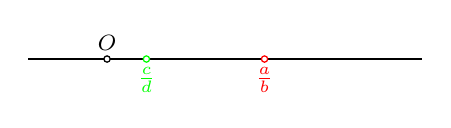
\begin{tikzpicture}
                    % \clip (0,0) rectangle (14.000000,10.000000);
                    {\footnotesize
                    
                    % Drawing segment A B
                    \draw [line width=0.016cm] (1.000000,1.500000) -- (1.960000,1.500000);%
                    \draw [line width=0.016cm] (2.040000,1.500000) -- (2.460000,1.500000);%
                    \draw [line width=0.016cm] (2.540000,1.500000) -- (3.960000,1.500000);%
                    \draw [line width=0.016cm] (4.040000,1.500000) -- (6.000000,1.500000);%
                    
                    % Marking point O by circle
                    \draw [line width=0.016cm] (2.000000,1.500000) circle (0.040000);%
                    \draw (2.000000,1.500000) node [anchor=south] { $O$ };%
                    
                    % Changing color 255 0 0
                    \definecolor{r255g0b0}{rgb}{1.000000,0.000000,0.000000}%
                    \color{r255g0b0}% 
                    
                    % Marking point \frac{a}{b} by circle
                    \draw [line width=0.016cm] (4.000000,1.500000) circle (0.040000);%
                    \draw (4.000000,1.500000) node [anchor=north] { $\frac{a}{b}$ };%
                    
                    % Changing color 0 255 0
                    \definecolor{r0g255b0}{rgb}{0.000000,1.000000,0.000000}%
                    \color{r0g255b0}% 
                    
                    % Marking point \frac{c}{d} by circle
                    \draw [line width=0.016cm] (2.500000,1.500000) circle (0.040000);%
                    \draw (2.500000,1.500000) node [anchor=north] { $\frac{c}{d}$ };%
                    \color{black}
                    }
                \end{tikzpicture}}    
            \end{block}}

            \only<4->{\begin{block}{}
                Slike pozitivnih racionalnih števil ležijo desno, slike negativnih racionalnih števil pa levo od koordinatnega izhodišča. \\
                \only<5->{\centering
                \begin{tikzpicture}
                    
                    % \clip (0,0) rectangle (14.000000,10.000000);
                    {\footnotesize
                    
                    % Drawing segment A B
                    \draw [line width=0.016cm] (1.000000,1.500000) -- (3.460000,1.500000);%
                    \draw [line width=0.016cm] (3.540000,1.500000) -- (6.000000,1.500000);%
                    
                    % Changing color 255 0 0
                    \definecolor{r255g0b0}{rgb}{1.000000,0.000000,0.000000}%
                    \color{r255g0b0}% 
                    
                    % Drawing segment B O
                    \draw [line width=0.016cm] (6.000000,1.500000) -- (3.540000,1.500000);%
                    
                    % Marking point pozitivna_tevila
                    \draw (4.750000,1.500000) node [anchor=north] { $pozitivna~ števila$ };%
                    \draw (4.750000,1.500000) node [anchor=south] { $\mathbb{Q}^+$ };%
                    
                    % Changing color 0 255 0
                    \definecolor{r0g255b0}{rgb}{0.000000,1.000000,0.000000}%
                    \color{r0g255b0}% 
                    
                    % Drawing segment O A
                    \draw [line width=0.016cm] (3.460000,1.500000) -- (1.000000,1.500000);%
                    
                    % Marking point negativna_tevila
                    \draw (2.250000,1.500000) node [anchor=north] { $negativna~ števila$ };%
                    \draw (2.250000,1.500000) node [anchor=south] { $\mathbb{Q}^-$ };%
                    
                    % Changing color 0 0 0
                    \definecolor{r0g0b0}{rgb}{0.000000,0.000000,0.000000}%
                    \color{r0g0b0}% 
                    
                    % Marking point O by circle
                    \draw [line width=0.032cm] (3.500000,1.500000) circle (0.040000);%
                    \draw (3.500000,1.500000) node [anchor=south] { $O$ };%
                    \color{black}
                    }
                \end{tikzpicture}}
            \end{block}}

            \only<6->{\begin{block}{}
                V množici ulomkov velja, da je vsak negativen ulomek manjši od vsakega pozitivnega ulomka.
            \end{block}}

        \end{frame}

        \begin{frame}
            \frametitle{Lastnosti relacije urejenosti}
            
            \only<2->{\begin{alertblock}{Monotonost vsote}
                \only<3->{Če na obeh straneh neenakosti prištejemo isto število, se neenakost ohrani.}
                \only<4->{$$ \mathbf{\frac{a}{b}<\frac{c}{d} \quad \Rightarrow \quad \frac{a}{b}+\frac{e}{f}<\frac{c}{d}+\frac{e}{f}} $$}
                % \only<5->{$$ \mathbf{p<q \quad \Rightarrow \quad p+r<q+r} $$}
            \end{alertblock}}

            \only<6->{\begin{alertblock}{Tranzitivnost}
                \only<7->{$$ \mathbf{\frac{a}{b}<\frac{c}{d} \quad \wedge \quad \frac{c}{d}<\frac{e}{f} \quad \Rightarrow \quad \frac{a}{b}<\frac{e}{f}} $$}
                % \only<8->{$$ \mathbf{p<q \quad \wedge \quad q<r \quad \Rightarrow \quad p<r} $$}
            \end{alertblock}}

        \end{frame}

        \begin{frame}

            \only<2->{\begin{alertblock}{}
                Pri množenju neenakosti s pozitivnim številom se znak neenakosti ohrani.
                \only<3->{$$ \mathbf{\frac{a}{b}<\frac{c}{d} \quad \wedge \quad \frac{e}{f}>0 \quad \Rightarrow \quad \frac{a}{b}\cdot\frac{e}{f}<\frac{c}{d}\cdot\frac{e}{f}} $$}
                % \only<4->{$$ \mathbf{p<q \quad \wedge \quad r>0 \quad \Rightarrow \quad p\cdot r<q\cdot r} $$}
            \end{alertblock}}

            \only<5->{\begin{alertblock}{}
                Pri množenju neenakosti s negativnim številom se znak neenakosti obrne.
                \only<6->{$$ \mathbf{\frac{a}{b}<\frac{c}{d} \quad \wedge \quad \frac{e}{f}<0 \quad \Rightarrow \quad \frac{a}{b}\cdot\frac{e}{f}>\frac{c}{d}\cdot\frac{e}{f}} $$}
                % \only<7->{$$ \mathbf{p<q \quad \wedge \quad r>0 \quad \Rightarrow \quad p\cdot r>q\cdot r} $$}
            \end{alertblock}}

            \only<8->{\begin{block}{}
                Pri prehodu na nasprotno vrednost se neenačaj obrne:
                \only<9->{$$ \mathbf{\frac{a}{b}<\frac{c}{d} \quad \Rightarrow \quad -\frac{a}{b}>-\frac{c}{d}} $$}
            \end{block}}



        \end{frame}

        \begin{frame}
            
            \only<2->{\begin{alertblock}{}
                Množica racionalnih števil pa je tudi \textbf{delno urejena}, in sicer z relacijo \textit{biti manjši ali enak} ($\leq$) oziroma \textit{biti večji ali enak} ($\geq$). Za ulomka $\frac{a}{b}$ in $\frac{c}{d}$ ($b,d\in\mathbb{N}$) velja vsaj ena izmed možnosti:
                \begin{enumerate}
                    \item<3-> prvi ulomek je večji ali enak od drugega $\frac{a}{b}\geq\frac{c}{d}$ natanko tedaj, ko je $ad\geq bc$;
                    \item<4-> drugi ulomek je večji ali enak od prvega $\frac{a}{b}\geq\frac{c}{d}$ natanko tedaj, ko je $ad\leq bc$;
                \end{enumerate}
            \end{alertblock}}

            \only<5->{\begin{block}{}
                Za (zgornjo) relacijo delne urejenosti veljajo naslednje lastnosti:
                \begin{itemize}
                    \item<6-> $\frac{a}{b}\leq\frac{a}{b}$ -- \textbf{refleksivnost};
                    \item<7-> $\frac{a}{b}\leq\frac{c}{d}  \wedge \frac{c}{d}\leq\frac{a}{b} \Rightarrow \frac{a}{b}=\frac{c}{d}$ -- \textbf{antisimetričnost} in
                    \item<8-> $\frac{a}{b}\leq\frac{c}{d}  \wedge \frac{c}{d}\leq\frac{e}{f} \Rightarrow \frac{a}{b}\leq\frac{e}{f}$ -- \textbf{tranzitivnost}.
                \end{itemize}
            \end{block}}


        \end{frame}

    \subsection{Algebrski ulomki}

        \begin{frame}
            \frametitle{Algebrski ulomki}
        \end{frame}

    \subsection{Računanje z ulomki}

        \begin{frame}
            \frametitle{Računanje z ulomki}
        \end{frame}

    \subsection{Potence s celimi eksponenti}

        \begin{frame}
            \frametitle{Potence s celimi eksponenti}
        \end{frame}

    \subsection{Pravila za računanje s potencami s celimi eksponenti}

        \begin{frame}
            \frametitle{Pravila za računanje s celimi eksponenti}
        \end{frame}

    \subsection{Premo in obratno sorazmerje}

        \begin{frame}
            \frametitle{Premo in obratno sorazmerje}
        \end{frame}

    \subsection{Odstotki}

        \begin{frame}
            \frametitle{Odstotki}
        \end{frame}


% \section{Realna števila, statistika}

\begin{frame}
    \sectionpage
\end{frame}

\begin{frame}
    \tableofcontents[currentsection, hideothersubsections]
\end{frame}

    \subsection{Realna števila}

        \begin{frame}
            \frametitle{Realna števila}
        \end{frame}

    \subsection{Kvadratni in kubični koren}

        \begin{frame}
            \frametitle{Kvadratni in kubični koren}
        \end{frame}

    \subsection{Intervali}

        \begin{frame}
            \frametitle{Intervali}
        \end{frame}

    \subsection{Absolutna vrednost}

        \begin{frame}
            \frametitle{Absolutna vrednost}
        \end{frame}

    \subsection{Sistem linearnih enačb}

        \begin{frame}
            \frametitle{Sistem linearnih enačb}
        \end{frame}

    \subsection{Obravnavanje linearnih enačb, neenačb, sistemov}

        \begin{frame}
            \frametitle{Obravnavanje linearnih enačb, neenačb, sistemov}
        \end{frame}

    \subsection{Absolutna in relativna napaka}

        \begin{frame}
            \frametitle{Absolutna in relativna napaka}
        \end{frame}

    \subsection{Sredine}

        \begin{frame}
            \frametitle{Sredine}
        \end{frame}

    \subsection{Razpršenost podatkov}

        \begin{frame}
            \frametitle{Razpršenost podatkov}
        \end{frame}

    \subsection{Prikazi}
        
        \begin{frame}
            \frametitle{Prikazi}
        \end{frame}

% \section{Pravokotni koordinatni sistem, linearna funkcija}

\begin{frame}
    \sectionpage
\end{frame}

\begin{frame}
    \tableofcontents[currentsection, hideothersubsections]
\end{frame}

    \subsection{Pravokotni koordinatni sistem}

        \begin{frame}
            \frametitle{Pravokotni koordinatni sistem}
        \end{frame}

    \subsection{Razdalja med točkama in razpolovišče daljice}

        \begin{frame}
            \frametitle{Razdalja med točkama in razpolovišče daljice}
        \end{frame}

    \subsection{Ploščina trikotnika}

        \begin{frame}
            \frametitle{Ploščina trikotnika}
        \end{frame}

    \subsection{Osnovno o funkcijah}

        \begin{frame}
            \frametitle{Osnovno o funkcijah}
        \end{frame}

    \subsection{Linearna funkcija in premica}

        \begin{frame}
            \frametitle{Linearna funkcija in premica}
        \end{frame}

    \subsection{Oblike enačbe premice}

        \begin{frame}
            \frametitle{Oblike enačbe premice}
        \end{frame}

    \subsection{Presešišče premic}

        \begin{frame}
            \frametitle{Presešišče premic}
        \end{frame}

    \subsection{Sistem linearnih neenačb}

        \begin{frame}
            \frametitle{Sistem linearnih neenačb}
        \end{frame}

    \subsection{Modeliranje z linearno funkcijo}

        \begin{frame}
            \frametitle{Modeliranje z linearno funkcijo}
        \end{frame}

    \subsection{(i) Linearno programiranje}
        
        \begin{frame}
            \frametitle{(i) Linearno programiranje}
        \end{frame}



\end{document}